


\documentclass[openany]{book}
\usepackage{fullpage}
\usepackage{makeidx}
\usepackage{graphicx}
\usepackage{ifthen}
\usepackage{listings}
\usepackage{color}
\usepackage{amsmath}  % for cases environment
\usepackage{amssymb}
\usepackage{comment}
\makeindex

\renewcommand{\topfraction}{0.999}
\renewcommand{\floatpagefraction}{0.999}
\renewcommand{\textfraction}{0.001}

% ====================================================================

\newcommand{\smart}{{\sc{S%
    \kern-.11em\raise.39ex\hbox{m}%
    \kern-.22em\raise.0ex\hbox{A}%
    \kern-.21em\raise.39ex\hbox{r}%
    \kern-.16em T}}}

\newcommand{\smartmeaning}{Stochastic Model-checking Analyzer for Reliability and Timing}

% For notes applying only to the current release
\newenvironment{release}{\color{blue}}{\color{black}}

% For shorter current release notes
\newcommand{\RELEASE}[1]{{\color{blue}#1}}

% For huge swaths of private text, including figures and other nasties
% However, the private environment cannot be nested.
\specialcomment{private}{\color{red}}{\color{black}}

% For undocumented features
\typein[\mantype]{Produce INTERNAL or EXTERNAL manual}
\ifthenelse{\equal{\mantype}{INTERNAL}}{%
  \newcommand{\PRIVATE}[1]{{\color{red}#1}}%   For short private sections
}{%
  \newcommand{\PRIVATE}[1]{}%
  \excludecomment{private}
}


% ====================================================================

\definecolor{dkgreen}{rgb}{0,0.6,0}
\definecolor{muave}{rgb}{0.58,0,0.82}

\lstdefinelanguage{smart}{%
  keywords={for,converge,guess},
  morecomment=[l]{//},
  morecomment=[s]{/*}{*/},
  morestring=[b]",
}

\lstdefinelanguage{output}{}

\lstset{frame=none,   % frame=tb,
  language=smart,
  % aboveskip=3mm,
  % belowskip=3mm,
  xleftmargin=2em,
  % xrightmargin=2em,
  showstringspaces=false,
  columns=flexible,
  basicstyle={\ttfamily},
  % basicstyle={\small\ttfamily},
  numbers=none,                     % line numbers
  keywordstyle=\underbar,
  commentstyle=\color{dkgreen},
  stringstyle=\color{muave},
  breaklines=true,
  breakatwhitespace=true,
  tabsize=2
}

% for SMART code
\newcommand{\Code}[1]{{\tt {#1}}}

% for command-line stuff
\newcommand{\Unix}[1]{{\tt {#1}}}


\newcommand{\Set}[1]{\mathcal{#1}}
\newcommand{\aset}{\Set{A}}           % absorbing states
\newcommand{\eset}{\Set{E}}           % event set
\newcommand{\nset}{\Set{N}}           % next state function (new set of states)
\newcommand{\pset}{\Set{P}}           % generic sat set
\newcommand{\qset}{\Set{Q}}           % generic sat set
\newcommand{\sset}{\Set{S}}           % reachability sets (global, local)
\newcommand{\tset}{\Set{T}}           % transient states

\newcommand{\pot}[1]{\widehat{#1}}    % potential (as opposed to actual)
\newcommand{\potsset}{\pot{\sset}}    % potential state space
\newcommand{\potnset}{\pot{\nset}}    % potential state space

\newcommand{\vect}[1]{\mathbf{#1}}    % does not bold lowercase greek
\newcommand{\gvect}[1]{\mbox{\boldmath{${#1}$}}} % wrong size for scripts
\newcommand{\vb}{\vect{b}}            % linear system constants
\newcommand{\vi}{\vect{i}}            % generic (from) state
\newcommand{\vj}{\vect{j}}            % generic (to) state
\newcommand{\vn}{\vect{n}}            % accumulated visits vector
\newcommand{\vs}{\vect{s}}            % generic state
\newcommand{\vp}{\vect{p}}            % probability vector
\newcommand{\vx}{\vect{x}}            % linear system unknowns
\newcommand{\initstate}{\vs^{init}}   % initial (starting) state
\newcommand{\vpi}{\gvect{\pi}}
\newcommand{\vsigma}{\gvect{\sigma}}

\newcommand{\matr}[1]{\mathbf{#1}}    % matrices
\newcommand{\0}{\matr{0}}            % the zero matrix
\newcommand{\A}{\matr{A}}             % generic linear system matrix
\newcommand{\I}{\matr{I}}             % the identity matrix
\renewcommand{\P}{\matr{P}}           % transition probability matrix
\newcommand{\Q}{\matr{Q}}             % infinitesimal generator matrix
\newcommand{\R}{\matr{R}}             % transition rate matrix


%%%%%%%%%%%%%%%%%%%%%%%%%%%%%%%%%%%%%%%%%%%%%%%%%%%%%%%%%%%%%%%%%%%%%%%%%%
% Numeric sets
\newcommand{\Reals}{\mathbb{R}}      % real numbers
\newcommand{\Naturals}{\mathbb{N}}   % natural numbers
\newcommand{\Integers}{\mathbb{Z}}   % integer numbers

%%%%%%%%%%%%%%%%%%%%%%%%%%%%%%%%%%%%%%%%%%%%%%%%%%%%%%%%%%%%%%%%%%%%%%%%%%
% Petri nets
\newcommand{\mk}[1]{{\framebox{#1}}}     % marking
\newcommand{\goesto}[1]{{\stackrel{#1}{\rightharpoondown}}} % firing 
\newcommand{\fires}[1]{\;\mbox{$[ #1 ]\!\!\! \Rightarrow$}\;} % firing, too
\newcommand{\PRE}{\succ}
\newcommand{\POST}{\succ\!\!\!\succ}

%%%%%%%%%%%%%%%%%%%%%%%%%%%%%%%%%%%%%%%%%%%%%%%%%%%%%%%%%%%%%%%%%%%%%%%%%%
% Logic symbols
\newcommand{\THEN}{\Rightarrow}                     % implication
\newcommand{\IFF}{\Leftrightarrow}                  % biimplication

%%%%%%%%%%%%%%%%%%%%%%%%%%%%%%%%%%%%%%%%%%%%%%%%%%%%%%%%%%%%%%%%%%%%%%%%%%
% CTL operators

\newcommand{\opA}{\mathsf{A}}                     % forall
\newcommand{\opE}{\mathsf{E}}                     % exists

\newcommand{\opF}{\mathsf{F}}                     % future
\newcommand{\opG}{\mathsf{G}}                     % globally
\newcommand{\opU}{\mathsf{U}}                     % until
\newcommand{\opX}{\mathsf{X}}                     % next

\newcommand{\opP}{\mathsf{P}}                     % past (reversed F)
\newcommand{\opH}{\mathsf{H}}                     % history (reversed G)
\newcommand{\opS}{\mathsf{S}}                     % since (reversed U)
\newcommand{\opY}{\mathsf{Y}}                     % reversed X

%%%%%%%%%%%%%%%%%%%%%%%%%%%%%%%%%%%%%%%%%%%%%%%%%%%%%%%%%%%%%%%%%%%%%%%%%%
% Miscellanea
\newcommand{\IGNORE}[1]{}                        % Ignore the argument
\newcommand{\TBD}[1]{\PRIVATE{{\bf TBD}: #1}}    % To Be Done 
\newcommand{\MSG}[1]{{\color{blue}#1}}    % messages
\newcommand{\SUPST}{\mbox{$^{\mathrm{st}}$}}     % to put a ^st in text
\newcommand{\SUPND}{\mbox{$^{\mathrm{nd}}$}}     % to put a ^nd in text
\newcommand{\SUPRD}{\mbox{$^{\mathrm{rd}}$}}     % to put a ^rd in text
\newcommand{\SUPTH}{\mbox{$^{\textrm{th}}$}}     % to put a ^th in text

\newcommand{\gfcstudent}{}
\newcommand{\gfcvisitor}{}

%%%%%%%%%%%%%%%%%%%%%%%%%%%%%%%%%%%%%%%%%%%%%%%%%%%%%%%%%%%%%%%%%%%%%%%%%%
% Temporary stuff to be eliminated
\definecolor{lightgrey}{rgb}{0.8,0.8,0.8}
\newcommand{\LIGHTGREY}[1]{\textcolor{lightgrey}{#1}}
\newcommand{\BLUE}[1]{\textcolor{blue}{#1}}

% ====================================================================

\begin{document}

\frontmatter

\begin{center}
\sf
% ~SMARTlogo~\\[8ex]
\mbox{\huge ~\hspace*{-2ex}{\smartmeaning}}
\\[4ex]
{\huge Version 3.2} \\[8ex]
{\huge \bfseries USER MANUAL} 

\vfill
  
{\large 
\begin{tabular}{l @{\hspace{1.5 in}} l}
   {\LARGE Design}   & {\LARGE Documentation} \\[0.3ex]
   Gianfranco Ciardo & Gianfranco Ciardo \\
   Andrew S.\ Miner  & Robert L.\ Jones, III \\
                     & Andrew S.\ Miner \\
                     & Radu I.\ Siminiceanu \\
                     & Min Wan \\[2ex]
\end{tabular}
}

\vfill

  ~ \\
  Iowa State University\\
  Department of Computer Science\\
  Ames, IA, 50011\\
  \{ciardo, asminer\}@iastate.edu\\
  http://smart.cs.iastate.edu
  
\vfill 

  Copyright \copyright 1996 --- 2008 Gianfranco Ciardo \\
  All rights reserved

\end{center}

\rm
\thispagestyle{empty}
\newpage

% ====================================================================

%
% $Id$
%

\section*{{\smart} overview and organization of this User Manual}

The {\smart} ({\smartmeaning}) tool is a software package to study complex
discrete-state systems. With {\smart}, it is possible to study the
logical behavior of the system, by generating the state space
underlying a complex model and asking temporal logic queries about
its dynamic behavior, as done in traditional model-checking.
Once one is satisfied that the logical behavior of the
system is both correct and correctly captured by the model,
performance, reliability, availability, and performability
measures about the system can be computed with a large variety of
state-of-the-art techniques.
{\smart} implements exact numerical solution algorithms,
approximate numerical solution algorithms,
and discrete-event simulation techniques.
These can be used in cooperation for the study of a complex
system, since multiple interacting models are supported in a
variety of ways, from a simple hierarchical solution of submodels
to a built-in fixpoint iteration mechanism which may be used to
perform sophisticated studies.
Numerical solution
algorithms are provided not only for the widely-used class of
models having an underlying continuous-time \index{Markov chain}Markov chain,
but also for the case where the underlying
process is a discrete-time Markov chain, or, under certain
conditions, even a Markov regenerative process arising from the
use of both discrete and continuous
\index{phase-type distribution}phase-type distributions in the same model.

\IGNORE{
A unifying language used to define the structure and the measures of models,
regardless of the formalism used to express them (queueing
networks, Markov chains, etc.) and of the type of study required
(performance, reliability, etc.);

Another way to deal with large and complex problems is the
use multiple processors.
This can be done in two ways
If several independent model solutions are needed, for example
to study a system under a range of different parameters,
they can be assigned to the available processors and run in parallel.
If, however, a single model is too large to be analyzed on a single processor
due to time or memory constraints, a more complex approach, using
a distributed algorithm, can be employed.
Both types of parallelism are available in {\smart}.
}

\begin{description}

\item{\bf Chapter \ref{SEC:Language}}
introduces the {\smart} input language used to define models and their
interactions.
Two types of low-level stochastic process formalisms
are presented, discrete-time and continuous-time
\index{Markov chain}Markov chains. High-level models expressed in
a formalism-specific way are instead presented in the following
individual chapters.

\begin{release}
Currently, the only high-level formalism supported by {\smart}
is an extended class of stochastic Petri nets.
More formalisms are planned for future versions.
\end{release}

\item{\bf Chapter \ref{SEC:SPN}}
describes how to define stochastic Petri nets models.
This is a very powerful and general formalism that can be used to model
discrete-state systems in virtually any domain.

\item{\bf Chapter \ref{SEC:SSGen}}
describes algorithms and options available to generate the state space
of a discrete-state model, regardless of the high-level formalism in which
it is expressed.
This fundamental step must occur before any model checking or
numerical solution activity.

\item{\bf Chapter \ref{SEC:ModelChecking}}
describes algorithms and options available to perform symbolic
model checking on a high-level model.

\item{\bf Chapter \ref{SEC:Numerical}}
describes algorithms and options available to solve the underlying
stochastic model numerically, using either traditional (explicit) or
symbolic (implicit) representations.

\begin{private}
\item{\bf Chapter \ref{SEC:Approximations}}
describes algorithms and options available to compute approximate
numerical solutions.
\end{private}

\begin{private}
\item{\bf Chapter \ref{SEC:Simulation}}
describes algorithms and options available to study models
using discrete-event simulation.
\end{private}

\item{\bf Chapter \ref{SEC:Examples}}
gives examples of {\smart} usage and reports runtimes and memory requirements
on them.

\item{\bf Appendix \ref{SEC:LanguageReference}}
lists the predefined types, functions, and options available in \smart.

\item{\bf Appendix \ref{SEC:BNF}}
formally defines the syntax of the {\smart} language using BNF notation.

\item{\bf Appendix \ref{SEC:PhaseType}}
gives key definitions and properties of
discrete and continuous phase-type distributions.

\item{\bf Release Notes}
at the end of this manual list information that a user of the current
release should know.
Other release-dependent information appears throughout this manual
\RELEASE{in blue text}.

\begin{private}
\item{\bf Internal Notes}
are designated throughout the manual for \smart{} developers or for 
work in progress.
This material is in red text and is omitted from the ``public'' user manual.
\end{private}

\end{description}

\vfill

\section*{\centering Acknowledgments}

The development of the techniques implemented in {\smart} has been partially
supported by the
National Aeronautics and Space Administration under grants
NAG-1-2168 and NAG-1-02095;
by the National Science Foundation under grants 
CSR-0546041, % Andy's CAREER
CCR-0219745, 
and
ACI-0203971;
by a joint STTR project with Genoa Software Systems,
Inc., for the Army Research Office;
and by the matching grant FED-95-011 from the Virginia Center for
Innovative Technology.
We are grateful to these organizations for making our research possible.

Any opinions, findings, and conclusions or recommendations expressed in this
material are those of the author(s) and do not necessarily reflect the views
of the National Science Foundation.



\tableofcontents

\mainmatter

% 
% $Id$
%

\chapter{The {\smart} language} \label{SEC:Language}
\markboth{THE SMART LANGUAGE}{}

This chapter introduces the {\smart} tool, its input language, and
its capabilities.
After an initial overview section, three main sections describe
how to define and manipulate deterministic quantities, random variables,
and stochastic processes, respectively.

%%%%%%%%%%%%%%%%%%%%%%%%%%%%%%%%%%%%%%%%%%%%%%%%%%%%%%%%%%%%%%%%%%%%%%
\section{Overview}

This section describes how to run {\smart} and the general structure of
{\smart} input files.
We adopt the convention of using a ``\Code{.sm}'' extension for the names
of these files, but this is not a requirement.

\subsection{Running {\smart}} 

Normally, {\smart} is run on one or more input files.
The command line used to run {\smart} on input file \Code{ff.sm} is
\lstset{language=bash}
\begin{lstlisting}
smart ff.sm
\end{lstlisting}
The input can also be partitioned over multiple files,
and it is possible to specify the standard input stream instead
of an ordinary file, by using ``\Code{-}''.
For example,
\begin{lstlisting}
smart ff1.sm ff2.sm - ff3.sm - ff4.sm
\end{lstlisting}
directs {\smart} to obtain input from file \Code{ff1.sm},
then file \Code{ff2.sm},
then the standard input (until the end-of-file is encountered),
then file \Code{ff3.sm}, then file \Code{ff4.sm}.
Note that the standard input stream is closed after finding the end-of-file,
thus the second \Code{-} specifier has no effect and files \Code{ff3.sm} and
\Code{ff4.sm} will not be able to read from standard input
(i.e., they cannot use functions that perform runtime input).


Running {\smart} with no arguments will display a help screen with version
information, as well as any command-line switches.
An important new feature of {\smart} is its built-in \emph{help} mechanism,
which may be invoked from the command line using the switch \Code{-h}.
For example,
\begin{lstlisting}
smart -h ctmc
\end{lstlisting}
will display documentation about the \Code{ctmc} formalism.

\subsection{Comments}

A {\smart} input file can contain comments.
Both single-line comments
\lstset{language=smart}
\begin{lstlisting}
int i := 1; // a single-line comment
\end{lstlisting}
and bracketed comments
\begin{lstlisting}
int i := 1; /* a bracketed
               comment */
\end{lstlisting}
can be used.
In the first case, the comment, starting from ``\Code{//}'' until the
end of the line, is ignored.
In the second case, the comment, starting from ``\Code{/*}'' until the
``\Code{*/}'', is ignored.


\subsection{\Code{\# include} directive}

{\smart} provides a file inclusion directive.
If a line
\begin{lstlisting}
#include "abc.sm"
\end{lstlisting}
appears anywhere in an input file (except within the quotes delimiting a string
or in a comment), the contents of file \Code{abc.sm} are read and used as if
they appeared in place of the \Code{include} line.

Inclusion directives can be recursively applied (i.e., an included file
can contain inclusion directives), as long as no circular
inclusions exist (e.g., if \Code{abc.sm} includes \Code{def.sm},
\Code{def.sm} cannot include \Code{abc.sm}).


\subsection{{\smart} statements}

A {\smart} input consists of a sequence of statements.
There are four classes of basic statements and two classes of
compound statements, which can be nested:
\begin{itemize}
\item
A {\bf \index{declaration}declaration} statement
is used to declare a \emph{function} of some set of \emph{parameters}.
As a special case, the set of parameters for a function can be empty,
thus the function is a constant.
In this sense, however, being ``constant'' should not to be confused with
being non-random (i.e., deterministic).
To ensure strict type-checking, the \emph{type} of the function and of
its parameters must be defined.  
\item
A {\bf \index{definition}definition} statement is used to
declare a function in the same
way declaration statements do, but it also specifies how to compute its value.
\item
An {\bf expression} statement is used to print the value of an expression,
although some function calls appearing in the expression
can also have side-effects,
such as generating output (see function \Code{print}),
or terminating the program (see function \Code{exit}).

\item
An {\bf option} statement is used to modify the behavior of {\smart}.
For example, there are options to control the solution algorithms (such
as the precision or the maximum number of iterations) or the level
of verbosity.
Options statements appear on a line beginning with ``\Code{\#}''
(the \Code{\# include} directive also begins with a ``\Code{\#}'', but it
should not be considered a statement).

\item
A \Code{for} compound statement is used to define arrays or to
repeatedly evaluate parametric expressions.
This is particularly useful for studies that explore how a result is
affected by a change in the modeling assumptions, such as the rate of
an event or the maximum size of a buffer.
\item
A \Code{converge} compound statement is used to specify a numerical fixpoint
iteration of the type often employed in conjuction with approximations.
\end{itemize}


\TBD{Rewrite this paragraph.}
The {\smart} language is strictly-typed, so objects belong to a \emph{type}:
\Code{void},
\Code{int},
\Code{bigint},
\Code{real},
\Code{bool}, or
\Code{string}.
All types are predefined, that is, dynamic definition of new types is not
possible, except for the creation of (multi-dimensional) arrays.
In addition to a type, an object also has a \emph{nature}, that is, it can
be a \emph{deterministic quantity} (the default),
a \emph{random variable}, or a \emph{stochastic process}.
For example, if we are modeling a computer system,
the number of processes waiting for the CPU as a function of time
is a stochastic process,
the number of processes waiting for the CPU at time 10 is a random
variable, and the average number of processes waiting for the CPU at time 10
is a deterministic quantity.
The following three sections describe how to specify deterministic quantities,
random variables, and stochastic processes.

%%%%%%%%%%%%%%%%%%%%%%%%%%%%%%%%%%%%%%%%%%%%%%%%%%%%%%%%%%%%%%%%%%%%%%
\section{Deterministic quantities}

The {\smart} language can be used to perform ``calculator-like'' computations.
It is important to become familiar with these simpler features of
the language before moving onto random variables and stochastic processes.

\subsection{A constant: $\pi$}

An example of a simple definition is
\begin{lstlisting}
real pi := 3.14;
\end{lstlisting}
which defines the constant \Code{pi} of type \Code{real} with value
\Code{3.14}.  Since the {\smart} language is declarative, not procedural,
the value of \Code{pi} is now set for the rest of its life.  A second
definition
\begin{lstlisting}
real pi := 3.1415;
\end{lstlisting}
causes an error.  Indeed, even a second occurrence of exactly the same
definition causes an error: each function can appear exactly once on
the left-hand side of a definition statement.
To query the value of \Code{pi}, we use an expression statement:
\begin{lstlisting}
pi;
\end{lstlisting}
which outputs the following line to the current output stream:
\lstset{language=output}
\begin{lstlisting}
3.14
\end{lstlisting}
\lstset{language=smart}
If we wanted a more informational output, we could format it
using the predefined function \Code{print}:
\begin{lstlisting}
print("The value of pi is ", pi, ".\n");
\end{lstlisting}
which would output the following line to the current output stream:
\lstset{language=output}
\begin{lstlisting}
The value of pi is 3.14.
\end{lstlisting}
\lstset{language=smart}






\subsection{A recursive one-parameter function: the factorial}
\label{SEC:factorial}

We can define a function to compute the factorial of an integer,
$n! = 1 \cdot 2 \cdot \ldots \cdot n$, as
\begin{lstlisting}
int fact(int n) := cond(n==0,1,n*fact(n-1));
\end{lstlisting}
The predefined function \Code{cond} returns the value of the second or
third parameter, according to whether the first parameter is \Code{true}
or \Code{false}, respectively.

We can call a function using either
\emph{named} parameter notation or with \emph{positional} parameter notation.
Thus, both \Code{fact(n:=7)} and \Code{fact(7)} evaluate to $7!$,
i.e., \Code{5040}.
The named parameter notation is especially useful to avoid errors and improve
readability when a function has many parameters.

\subsection{Arrays: the first ten factorial numbers}

The definition of function \Code{fact} does not
cause any computation to be performed.
To compute and output the value of the
first ten factorial numbers, we can use a \Code{for} statement:
\begin{lstlisting}
for (int i in {0..9}) {
  fact(n:=i);
}
\end{lstlisting}
but doing so requires the computation of each factorial number ``from scratch''.
A better way to do this is to use an array \Code{f} indexed by an
\emph{iterator} \Code{i}:
\begin{lstlisting}
for (int i in {0..9}) {
  int f[i] := cond(i==0,1,i*f[i-1]);
  f[i];
}
\end{lstlisting}
This defines an array \Code{f} with an index set from \Code{0} to \Code{9},
with a step of one (the default).  To refer to a particular value computed
inside a \Code{for} statement from a subsequent statement, the traditional
``square brackets'' notation is used.  
This definition is the most efficient, since it requires only nine
multiplications in total.
However, it computes only the first ten factorial numbers:
it does not help if we need to compute $12!$.

A fundamental observation is appropriate at this point.
Since {\smart} does not evaluate a function until its value is required in
output, our array-based definition of the first ten factorial numbers
is just as efficient when written as
\begin{lstlisting}
for (int i in {9..0..-1}) {
  int f[i] := cond(i==0,1,i*f[i-1]);
}
for (int i in {9..0..-1}) {
  f[i];
}
\end{lstlisting}
that is, if we were counting \Code{i} down from 9 to 0
(the step is explicitly specified to be \Code{-1} in
the above \Code{for} statements).
Note, however, that
\begin{lstlisting}
for (int i in {9..0..-1}) {
  int f[i] := cond(i==0,1,i*f[i-1]);
  f[i];
}
\end{lstlisting}
would result in an error message because it attempts to output
\Code{f[i]}, which requires the value of \Code{f[i-1]}, before
\Code{f[i-1]} has been defined.





\subsection{Managing large integers}

Ordinary \Code{int} quantities can only store quantities in a limited
range, $[-2^{31},2^{31}-1]$ on 32-bit architectures
and $[-2^{63}, 2^{63}-1]$ on 64-bit architectures.
In \smart, much larger integers have to be manipulated at times,
thus an ``arbitrary-size integer'' type, \Code{bigint}, is provided as well.
For example, if we define the two factorial functions
\begin{lstlisting}
bigint bfact(int n) := cond(n==0,1,bfact(n-1)*n);
int    ifact(int n) := cond(n==0,1,ifact(n-1)*n);
\end{lstlisting}
the \Code{for} statement
\begin{lstlisting}
for (int i in {1..20}) {
  print("ifact(",i:2,") = ",ifact(i):11,"    bfact(",i:2,") = ",bfact(i),"\n");
}
\end{lstlisting}
would produce, in output,
\begin{lstlisting}
ifact( 1) =           1    bfact( 1) = 1
ifact( 2) =           2    bfact( 2) = 2
ifact( 3) =           6    bfact( 3) = 6
...
ifact(10) =     3628800    bfact(10) = 3,628,800
ifact(11) =    39916800    bfact(11) = 39,916,800
ifact(12) =   479001600    bfact(12) = 479,001,600
ifact(13) =  1932053504    bfact(13) = 6,227,020,800
...
ifact(19) =   109641728    bfact(19) = 121,645,100,408,832,000
ifact(20) = -2102132736    bfact(20) = 2,432,902,008,176,640,000
\end{lstlisting}
%ifact( 1) =           1    bfact( 1) = 1
%ifact( 2) =           2    bfact( 2) = 2
%ifact( 3) =           6    bfact( 3) = 6
%ifact( 4) =          24    bfact( 4) = 24
%ifact( 5) =         120    bfact( 5) = 120
%ifact( 6) =         720    bfact( 6) = 720
%ifact( 7) =        5040    bfact( 7) = 5,040
%ifact( 8) =       40320    bfact( 8) = 40,320
%ifact( 9) =      362880    bfact( 9) = 362,880
%ifact(10) =     3628800    bfact(10) = 3,628,800
%ifact(11) =    39916800    bfact(11) = 39,916,800
%ifact(12) =   479001600    bfact(12) = 479,001,600
%ifact(13) =  1932053504    bfact(13) = 6,227,020,800
%ifact(14) =  1278945280    bfact(14) = 87,178,291,200
%ifact(15) =  2004310016    bfact(15) = 1,307,674,368,000
%ifact(16) =  2004189184    bfact(16) = 20,922,789,888,000
%ifact(17) =  -288522240    bfact(17) = 355,687,428,096,000
%ifact(18) =  -898433024    bfact(18) = 6,402,373,705,728,000
%ifact(19) =   109641728    bfact(19) = 121,645,100,408,832,000
%ifact(20) = -2102132736    bfact(20) = 2,432,902,008,176,640,000
on a 32-bit machine.
Note that the \Code{int} factorial overflows from \Code{13} on,
so that the returned values are incorrect, and can even be negative,
as \Code{ifact(20)} illustrates.
{\smart} does not raise an error when an overflow happens:
this is unfortunate, but it is common integer behavior
in modern programming languages.

Using a \Code{bigint} instead of an \Code{int} ensures that the
correct value is computed, but incurs a substantial overhead.
Thus, {\smart} uses ordinary integers for its normal internal operations,
and the \Code{bigint} type should be used only when needed.
It is the responsibility of the user to decide when this is the case.

\TBD{Need to discuss ``\Code{,}'' in formatting of \Code{bigint}}


\begin{comment}
\subsection{A \Code{real} iterator}

\TBD{Is this something we want to forbid from future versions?
In restrospect, it might be more trouble than it is worth it...}

Array iterators can be of type \Code{real}, as in the following
example defining a three-element array \Code{y}:
\begin{lstlisting}
for (real x in {O.1,O.2,0.4}) {
  real y[x] := 3*x*x;
}
\end{lstlisting}
Care must be taken to avoid indexing errors due to the finite precision of
floating-point arithmetic.  
To address this problem, {\smart} considers two floating-point indices to be
equal if they are within an absolute or relative precision $\delta$.
In the above example, {\smart} evaluates the expression \Code{y[x]} to 
\Code{y[0.1]} for any value of \Code{x} satisfying 
\[
  \begin{array}{c@{~~~~}l}
     0.1-\delta \leq \Code{x} \leq 0.1+\delta
     & 
     \mbox{if absolute precision is used,}
     \\
     0.1-0.1\delta \leq \Code{x} \leq 0.1+0.1\delta
     &
     \mbox{if relative precision is used.}
  \end{array}
\]
The value of $\delta$ is dictated by the option \Code{IndexPrecision}
(with a default of $10^{-5}$) and the
type of precision test is dictated by the option \Code{IndexPrecisionTest}
(with default value \Code{RELATIVE}, the other possible value
being \Code{ABSOLUTE}).
Thus, if the options are set using the statements
\begin{lstlisting}
# IndexPrecisionTest ABSOLUTE
# IndexPrecision  0.015
\end{lstlisting}
then the expression \Code{y[0.099]} evaluates to \Code{0.03}, and the
expression \Code{y[0.08]} results in a ``range error'' message,
and evaluates to \Code{null}.
\end{comment}





\subsection{Specifying numeric sets to be used in \Code{for} statements}

A numeric set of \Code{int} or \Code{real} values can be specified by explicitly
listing its elements, e.g., \verb%{3,4,7}% or \verb%{0.3,0.4,0.7}%.
The type of a set defined this way is \verb%{int}% if each of its elements
is an \Code{int}, \verb%{real}% if each of its elements is a \Code{real}.
No mixing of \Code{int} and \Code{real} elements is allowed.  

\begin{comment}
The type of a set defined this way is \verb%{int}% if each of its elements
is an \Code{int}, \verb%{real}% if any of its elements is a \Code{real}.
Thus, for example, \verb%{3,4,7.0}% is of type \verb%{real}%.
\end{comment}

It is also possible to specify a range of elements, instead of a single
element,  when defining a set.
A range has the syntax \Code{$first$..$upper$..$step$} and is equivalent
to explicitly specifying the elements $first$, $first+step$,
$first+step+step$, and so on, up to, but not included, the first element
that exceeds $upper$.
Exceptions: if $step$ evaluates to $0$, the range identifies the single
element $first$ while, if $first > upper$ and $step > 0$,
or $first < upper$ and $step < 0$, the range identifies no elements at all;
in either case {\smart} issues a warning message.
The type of the elements identified by a range
is \Code{real} if $first$, $upper$, or $step$ is \Code{real},
it is \Code{int} otherwise.
When $first$ and $upper$ have type \Code{int}, $step$ can be omitted:
it defaults to \Code{1}, thus \Code{3..7} is equivalent to \Code{3..7..1},
they both identify the elements \Code{3,4,5,6,7}.
However, it is an error to omit the $step$ when $first$ or $upper$
have type \Code{real}.
It is possible to mix the two modes of set specification, as in
\verb%{1,3,5..10,20..50..5}%.
Care must be taken when using \Code{real} ranges, due to the finite
precision of floating point numbers:
\Code{\{0.1..0.9..0.1\}} might specify either eight or nine \Code{real}
elements, depending on whether the result of summing
nine values \Code{0.1} is greater than \Code{0.9} or not,
when these quantities are represented as floating-point numbers
(one could specify \Code{\{0.1..0.91..0.1\}} to ensure that the range
contains exactly nine elements).
\begin{comment}
As expected, the type of the set is \verb%{real}% if any of the elements
specified has type \Code{real}, otherwise it is \verb%{int}%.
\end{comment}

While not, strictly speaking, a set property, the order in which the elements
are specified in the set is important in {\smart};
for example, it affects the order in
which a \Code{for} statement is executed.
In turn, this order can affect correctness or efficiency.
{\smart} respects the order specified by the user, so, for example,
\verb%{-3..0}% and \verb%{0..-3..-1}% represent the same set,
but with the elements in reverse order.
Note that it is not an error to specify the same element multiple times
in a set, but any subsequent specification is ignored.
Thus, the two set specifications \verb%{1,3,2..6,4,8}% and
\verb%{1,3,2,4,5,6,8}% are exactly equivalent, with respect to both the
elements they contain and their order.

\TBD{We might want to drop sets of reals...}

\TBD{Discuss: braces are also used to collect void expressions into sequences.}




\subsection{Nested \Code{for} statements}

Since \Code{for} statements can be nested, the dimensionality of a
declaration is determined by the sequence of iterators, from the
outermost to the innermost.  For example,
\begin{lstlisting}
for (int n in {1,2}) {
  for (int k in {1..5}, int i in {3,7,5}) {
    real g[n][k][i] := 0.2*n*k*i;
  }
}
\end{lstlisting}
defines a tridimensional ($2 \times 5 \times 3$)
array \Code{g} of \Code{real} constants.
Note that the scope of the iterators in a \Code{for} statement is local to that
statement and to those included in it.

It is an error to define objects with a smaller dimensionality than that
corresponding to the enclosing \Code{for} statements, or with indices
in an order other than that in which they appear as iterators
Thus, the definition of \Code{h} in
\begin{lstlisting}
for (int i in {0..9}, int j in {0..9}) {
  int h[i] := ...;
  int f[i][j] := ...;
  int g[j][i] := ...;
}
\end{lstlisting}
is illegal because it does not have index \Code{j}, while the definition
of \Code{g} is illegal because index \Code{i} follows index \Code{j}.

Analogously, it is illegal
to define functions with parameters within a \Code{for} statement,
such as \Code{fact} in the following:
\begin{lstlisting}
for (int i in {0..9}) {
  int fact(int n) := cond(n==0,1,n*fact(n-1));
  int f[i] := fact(i);
}
\end{lstlisting}
This is because such a function would be either independent of the
iterators (as \Code{fact} is in the above example), or
dependent on them;
in the former case, it could be specified outside the \Code{for} statement,
in the latter the semantic of calling it from outside the \Code{for}
statement would be undefined, since the iterators have no value
outside the \Code{for} statement.


\subsection{Parameter defaults}

Normally, each formal parameter in the definition of a function must
correspond to an actual parameter in a function call.
However, it is possible to set default values for the formal parameters.
If we define
\begin{lstlisting}
int f2(int a:=1, int b) := a*b;
\end{lstlisting}
the function calls \Code{f2(a:=1,b:=3)}, \Code{f2(1,3)},
\Code{f2(a:=default,b:=3)}, \Code{f2(default,3)}, or \Code{f2(b:=3)} are
exactly equivalent.
However, the call \Code{f2(3)} is illegal: named
parameters must be used if some parameters are not listed explicitly.

Note that it is possible to define a default value for each parameter
of a function, but it is not possible to call that function with an
implicit default for all of its parameters
(i.e., at least one of them must be set to \Code{default} explicitly),
since the function must be invoked with named parameters.

\begin{comment}
\subsection{A parallelizable \Code{for} statement}

The \Code{for} statement is a natural candidate for parallelization.
Indeed, {\smart} can recognize parallelism and perform
the concurrent computation of all the values specified in a \Code{for}
statement, provided no dependencies from one ``iteration'' to the next exist,

For example, the 100 values
\begin{lstlisting}
for (int i in {0..9}, int j in {0..9}) {
  int measure[i][j] := mymodel(i,j);
}
\end{lstlisting}
can be computed concurrently,
This reduces the total execution time in cases where the solution of
\Code{mymodel}
requires substantial computation, and multiple processors are available.
Such situations are common in parametric modeling studies.
\end{comment}

\subsection{Overloading: a \Code{real} factorial} \label{SEC:realFactorial}

The {\smart} language allows identifier overloading.
The same identifier can be used to define multiple functions, as long as
the order, type, or name of the formal parameters can be used to
distinguish which one is meant by a function call.  For example, we
could define both an ``integer factorial'' and a ``real factorial'':
\begin{lstlisting}
int  fact(int  n) := cond(n<1,1  ,n*fact(n-1));
real fact(real n) := cond(n<1,1.0,n*fact(n-1));
\end{lstlisting}
Then, \Code{fact(8)} and \Code{fact(5.4)} would call the standard
(integer) factorial or the real factorial, respectively.

\begin{comment}
Overloading also applies to arrays.  If we defined
\begin{lstlisting}
for (int i in {0..9}) {
  real f[i] := i * 1.0;
}
for (real i in {1.0..9.0..1.0}) {
  real f[i] := i * 10.0;
}
\end{lstlisting}
the expressions \Code{f[2]} and \Code{f[2.0]} would refer to the first and
second array, respectively.
\end{comment}
Furthermore, we can define arrays and functions with the same name;
these are distinguished at the syntactical level by the use of
``\Code{[]}'' or ``\Code{()}'', respectively.

As always, common sense should be followed:
overloading can be helpful when used judiciously, but it can become confusing
when overused, and it can lead to ambiguous function calls altogether.
For example, if we have defined the functions
\begin{lstlisting}
int f(real y) := ... ;
int f(real x) := ... ;
\end{lstlisting}
we can distinguish between them with the named parameter calls
\Code{f(x:=1.0)} and \Code{f(y:=1.0)}, but {\smart} rejects the positional
parameter call \Code{f(1.0)} as illegal.
Conversely, the functions
\begin{lstlisting}
int f(real x, int i) := ... ;
int f(int i, real x) := ... ;
\end{lstlisting}
cannot be distinguished if we use the named parameter call
\Code{f(x:=3.1,i:=1)}, but can be
distinguished if we use the positional calls \Code{f(3.1,1)}
and \Code{f(1,3.1)}.
For analogous reasons, the functions
\begin{lstlisting}
int f(int i:=1) := ... ;
int f(real x:=2) := ... ;
\end{lstlisting}
cannot be called using \Code{f(default)}.
Finally, the type returned by a function cannot be used to resolve ambiguities
due to overloading, thus, when {\smart} reads the second definition for \Code{f}
in
\begin{lstlisting}
int f(int x):= ... ;
real f(int x):= ... ;
\end{lstlisting}
it will issue an error message and ignore it.




\subsection{Type promotions: manual or automatic?}

\TBD{Update this; especially to include automatic promotions
of functions (adding proc and rand as necessary)}

\begin{table}
\renewcommand{\arraystretch}{0.97}
\begin{center}\begin{tabular}{| l | l |}
\hline
\multicolumn{1}{| c |}{\bf Original type} &
\multicolumn{1}{  c |}{\bf Promoted type} \\
\hline
\hline
\Code{int              }&\Code{real}\\
\Code{int              }&\Code{bigint}\\
\Code{bigint           }&\Code{real}\\
\Code{rand int         }&\Code{rand real}\\
\Code{proc int         }&\Code{proc real}\\
\hline
\Code{bool             }&\Code{rand bool}\\
\Code{int              }&\Code{ph int}\\
\Code{ph int           }&\Code{rand int}\\
\Code{real             }&\Code{rand real}\\
\Code{ph real          }&\Code{rand real}\\
\hline
\Code{rand bool        }&\Code{proc bool}\\
\Code{rand int         }&\Code{proc int}\\
\Code{rand real        }&\Code{proc real}\\
\hline
\Code{proc bool        }&\Code{bool}\\
\Code{proc int         }&\Code{int}\\
\Code{proc real        }&\Code{real}\\
\hline
\end{tabular}\end{center}
\caption{Automatic type promotions.}
\label{TAB:typePromotions}
\end{table}

Assume that we defined an integer constant \Code{k}, and we now want
to call the real factorial function with \Code{k} as the actual
parameter.  One reason for wanting to do this is that, if \Code{k} is
large, the integer factorial function might result in an overflow,
while the value real factorial might still fit in the floating point
representation of the machine.

We can force an automatic conversion by summing a (real) zero to
\Code{k}, as in \Code{fact(k+0.0)}.  This method works, but is inelegant;
a much better way is to use an explicit type conversion, \Code{fact(real(k))}.

For simplicity's sake, promotions such as the \Code{int}-to-\Code{real}
promotion for \Code{int k} in the expression \Code{k+0.0}, occur automatically.
Table \ref{TAB:typePromotions} lists the automatic
type promotions that can take place when evaluating an expression.
Other promotions must be explicitly requested
using the syntax \Code{new\_type(variable)}, where it must be possible
to promote the type of \Code{variable} to \Code{new\_type}.
In addition to the automatic promotions of Table \ref{TAB:typePromotions},
the legal explicit promotions are
from \Code{bigint} to \Code{int} and from \Code{real} to \Code{int}
or to \Code{bigint}.
Note that \Code{int(x)} and \Code{bigint(x)} discard the decimal portion of
the real value \Code{x} while, if rounding to the closest integer is desired,
\Code{round(x)} should be used instead.
Functions \Code{floor} and \Code{ceiling} are also available.
For example,
\Code{int(3.2)},
\Code{floor(3.2)}, and
\Code{round(3.2)} evaluate to \Code{3}, while
\Code{ceiling(3.2)} evaluates to \Code{4};
\Code{int(-3.2)},
\Code{round(-3.2)},
and \Code{ceiling(-3.2)}
evaluate to \Code{-3}, while
\Code{floor(-3.2)}, evaluates to \Code{-4}.





We observe that the \Code{real}-to-\Code{int} and \Code{bigint}-to-\Code{int}
conversions cause an overflow if the value to be converted does not fit
in an \Code{int} type;
indeed, even the \Code{bigint}-to-\Code{real} conversion can overflow,
since a \Code{bigint} can have thousands of digits 
({\smart} issues a warning message in this case, and the value of
the converted expression is set to \Code{null}).

Also, casting an \Code{int} or \Code{bigint} into a \Code{real}
may cause loss of precision, since the number of bits for the mantissa
is fixed to a relatively small number in the internal representation
of a \Code{real} (of course, no warning is issued in this case).

Promotion of the actual parameters in a function call or of the
expressions used to index an array, however, requires special
attention, because of the possible ambiguities arising from
overloading.  Consider for example the definitions
\begin{lstlisting}
real x(int i, real j) := ... ;
real x(real i, int j) := ... ;
\end{lstlisting}
The function calls \Code{x(1,1.0)} and \Code{x(1.0,1)} clearly refer to
the first and second definitions, respectively.  The call \Code{x(1,1)},
however, could refer to either, depending on whether the first or the
second actual parameter is promoted to \Code{real}.
{\smart} first attempts to find a function or array requiring no promotion at
all, that is, a function or array for which the formal parameters or indices
exactly match the actual parameters or indices used in the expression.
Only if this fails is promotion attempted.
If there are multiple choices for promoting the set of parameters,
{\smart} searches for a unique choice that requires promoting the minimum
number of parameters: if there is such a function or array, it is chosen;
otherwise, {\smart} issues an error message.
The option \Code{ParameterWarnings} controls under what conditions a warning is
issued when {\smart} automatically promotes parameters in function calls
(see section \ref{SEC:smart-options}).

\begin{comment}
Finally, note that a set of integers, \Code{\{int\}}, cannot be promoted
(neither automatically nor explicitly) to a set of reals, \Code{\{real\}}.
Thus, in the following, the former works but the latter is an error:
\begin{lstlisting}
for (real r in {1..5..1.0}) { ... }
for (real r in {1..5..1})   { ... }
\end{lstlisting}
\end{comment}


\subsection{Using iterator values to define iterators}

The value of an iterator can be used to define the value of further inner
iterators:
\begin{lstlisting}
for (int x in {1..9}, int y in {x*2,x**,x*8}) {
  int v[x][y] := x*y;
}
\end{lstlisting}

Syntactically, the iterators of a \Code{for} statement must always be
scalars: \Code{y} depends on \Code{x} in the above examples, but its
dependency is implicit.
In other words, it is an error to write
\begin{lstlisting}
for (int x in {1..9}, int y[x] in {x*2,x*4,x*8}) {
  int v[x][y[x]] := x*y[x];
}
\end{lstlisting}

\subsection{The \Code{null} value}

Our real factorial function defined in Section \ref{SEC:realFactorial} 
returns \Code{1} if it is called with a negative argument.
The integer factorial defined in Section
\ref{SEC:factorial} has an even worse behavior: it goes into an
infinite recursion if it is called with a negative argument.  
To prevent these problems, we can use the special value \Code{null}, and
modify our factorials as follows:
\begin{lstlisting}
int  fact(int n)  := cond(n<0,null,cond(n==0,1,  n*fact(n-1)));
real fact(real n) := cond(n<0,null,cond(n<1, 1.0,n*fact(n-1))); 
\end{lstlisting}

Any expression where one of the operands is \Code{null},
such as \Code{null+3} or \Code{sqrt(fact(-2))} also evaluates
to \Code{null}.
The only way an expression evaluating to \Code{null} can be meaningfully
used is if it is used as the argument of a function call, and the function
knows how to deal with a \Code{null} value.
The predefined function \Code{cond}, for example,
simply returns the value of the second or third parameter; if the
selected one is \Code{null}, so is the returned value.  The same holds
for the predefined function \Code{case}.
The predefined function \Code{is\_null} is also available:
it returns \Code{true} or \Code{false}
according to whether its argument has value \Code{null} or not.

Some expressions or functions might also evaluate to \Code{null}.
For example, \Code{1/0} is undefined because we cannot determine its
sign (see the next section, which discusses infinite values), thus
it evaluates to \Code{null}.
Analogoulsy, \Code{pow(-3,2.5)} is undefined because the base of the power
function must be non-negative if the exponent is real, thus it also
evaluates to \Code{null};
however, \Code{pow(-3,2)} is legal and evaluates to \Code{9}.

\subsection{Managing \Code{infinity}}

{\smart} allows an \Code{int} or \Code{real} function to have an infinite value.
The predefined \Code{int} value \Code{infinity} can be used for this purpose.
The sign of \Code{infinity} is positive, thus we can express a negative
infinite value by negating it.
Since \Code{int} values can be promoted to \Code{real}, real
values can have an \Code{infinity} value as well:
\begin{lstlisting}
int positive_infinity := infinity;
int negative_infinity := -infinity;
real x := negative_infinity;
\end{lstlisting}
Operations involving \Code{infinity} are defined as expected.
For example, the following expressions are legal:
\begin{lstlisting}
-infinity + infinity * (-5) + 72;      // -infinity (of type int)
-infinity / -3.4;                      // infinity (of type int)
infinity > -infinity;                  // true
pow(3,7.2*infinity);                   // infinity (of type real)
\end{lstlisting}
However, operations such as the following ones are undefined
({\smart} returns \Code{null} and issues a warning):
\begin{lstlisting}
infinity - infinity;
0 * infinity;                     
infinity >= infinity;
3.2/0;
pow(-3,infinity);
mod(3,infinity);
mod(infinity,3);
\end{lstlisting}
When printing an \Code{int} or \Code{real} value that evaluates to
\Code{infinity}, {\smart} uses the value of the option \Code{InfinityString},
which has a default value of \Code{"infinity"}.
This affects only the way an infinite value is written to output,
not the way it must occur in input.
Thus, for example, the input file
\begin{lstlisting}
# InfinityString "oo"
print(0,",",1,",",2,",...,",infinity,"\n");
\end{lstlisting}
produces the output
\begin{lstlisting}
0,1,2,...,oo
\end{lstlisting}


\subsection{Fixpoint iterations: solving $x = \sqrt{x}$}

An important feature of {\smart} is its ability to use numerical fixpoint
iterative solutions, where multiple parametric models are solved repeatedly.
The approach starts with initial guesses for their parameters, and successively
refines them, until convergence within a given precision is achieved,
or a maximum number of iterations is reached.
For example, we can find the zero $x=1$ for the expression
$x - \sqrt{x}$ by transforming it into the fixpoint equation $x = \sqrt{x}$,
and starting with any positive guess for $x$:
\begin{lstlisting}
converge {
  real x guess 100;
  real x := sqrt(x);
}
\end{lstlisting}
The value of \Code{x} after the \Code{converge} statement is the computed
fixpoint value.  The precision $\epsilon$ to which this value is
computed can be changed in an option statement.  The iterations are
stopped when two subsequent values for \Code{x} are within a relative or
absolute precision of $\epsilon$ (note that this does not guarantee that 
\Code{x} is within $\epsilon$ of the true fixpoint solution), or when the
number of iterations exceeds the maximum number of allowed iterations 
defined by the option \Code{MaxConvergeIters}.
Similar to the case of array index precision, the converge precision $\epsilon$ 
and the type of precision used are determined by the options 
\Code{ConvergePrecision} and \Code{ConvergePrecisionTest}.
Note that the statement providing an initial guess for \Code{x}
is a declaration: the definition of \Code{x} must also appear in the
body of the \Code{converge} statement.
However, unlike ordinary declarations, at most one \Code{guess} statement
can appear for each \Code{x} before the definition of \Code{x},
and none after.
Only \Code{real} objects can be defined inside a \Code{converge}
statement.

If any variable being iterated upon by the \Code{converge} statement becomes
\Code{null}, it will remain \Code{null} regardless of the values it might
be assigned in further iterations.
Thus, for example, if we wanted to find the zero of $x - \sqrt{x+1}$
but misstyped ``\Code{x-1}'' instead of ``\Code{x+1}'' in the following
\begin{lstlisting}
converge {
  real x guess 10;
  real x := sqrt(x-1);
}
\end{lstlisting}
the subsequent values assumed by \Code{x} would be
\Code{3}, which is  \Code{sqrt(10-1)}, then
\Code{1.41421}, which is \Code{sqrt(3-1)}, then
\Code{0.64359}, which is \Code{sqrt(1.41421-1)}, and finally
\Code{null}, since \Code{sqrt(0.64359-1)} is undefined.

We stress that, unlike the \Code{for} statement, the \Code{converge}
statement does not affect the dimensionality of the objects declared in it.



\subsection{Multi-variable fixpoint iterations} \label{SEC:multconv}

In practice, most fixpoint iterations involve several variables and
complex dependencies among them.
Consider the fixpoint iteration
\begin{lstlisting}
converge {
  real d guess 0.5;
  real b guess 0.3;
  real a guess 0.2;
  real c guess 0.7;
  real c := fc(d,b);
  real b := fb(d,c);
  real a := fa(b,c);
  real d := fd(a);
}
\end{lstlisting}
The dependency graph of Fig.~\ref{FIG:NestedDep} represents this
situation.  An arc from $x$ to $y$ signifies that the value of $y$
depends on the value of $x$.  

In this \Code{converge} statement, iterations continue until
subsequent values for \Code{a}, \Code{b}, \Code{c}, and \Code{d} differ by
less then $\epsilon$.
If the option \Code{UseCurrent} is set to \Code{true} (this is the default),
the newly computed values are used immediately, otherwise,
the newly computed values are not used until the next iteration.  
In our example, the computation of \Code{b}, \Code{a}, and \Code{d} is
affected by this choice:
with \Code{UseCurrent} set to \Code{true}, the calls
\Code{fb}, \Code{fa}, and \Code{fd} use the most recent values
available for their arguments.

{\smart} determines whether enough guesses are provided to start the iterations.
The rule is simple: any variable appearing on the right
side of an assignment statement must have a value when the statement
is executed.  If such a variable has not yet been defined, then it
must be given an initial guess.  If the option \Code{UseCurrent} is set
to \Code{false}, then every variable appearing on the right side of an
assignment must be given an initial guess.
Thus, in our example, the initial guesses for \Code{a} and \Code{c} are
required when \Code{UseCurrent} is set to \Code{false}, while 
they are not necessary (and are ignored) when \Code{UseCurrent}
is set to \Code{true}.

\subsection{Nested fixpoint iterations}

It is often advisable to nest fixpoint iterations.
For instance, in the \Code{converge} statement shown in the previous
section, we might know that \Code{b} and \Code{c}
require many iterations to stabilize, but that, fortunately, each call
to \Code{fb} and \Code{fc} requires little computation.  Then, the
following nested scheme might be advantageous:
\begin{lstlisting}
# UseCurrent true
converge {
  real d guess 0.5;
  real b guess 0.3;
  converge {
    real c := fc(d,b);
    real b := fb(d,c);
  }
  real a := fa(b,c);
  real d := fd(a);
}
\end{lstlisting}
Now, the values of \Code{b} and \Code{c} are iterated upon
until they stabilize, for each updated guess for \Code{d}.

Note that the position of the statement \Code{real b guess 0.3} causes
the guess \Code{0.3} to be used only once: the first time the innermost
\Code{converge} statement is executed.  The subsequent inner fixpoint
iterations performed whenever the value of \Code{d} is updated will use the
latest value for \Code{b}, not \Code{0.3}.  The alternative behavior, where
\Code{b} is set to \Code{0.3} every time the innermost \Code{converge}
statement is reached, can be obtained by moving the statement
\Code{real b guess 0.3} inside the innermost \Code{converge} statement,
but this would probably worsen the convergence behavior.

\begin{figure}
  \centering
  \includegraphics[scale=0.75]{figures/NestedDep.pdf}
  \caption{A \Code{converge} dependency graph.}
  \label{FIG:NestedDep}
\end{figure}

\subsection{Nested \Code{for} and \Code{converge} statements}

A \Code{for} statement can contain a \Code{converge} statement, as in
\begin{lstlisting}
for (int i in {0..5}) {
  converge {
    real x[i] guess 100;
    real x[i] := sqrt(x[i] + i);
  }
}
\end{lstlisting}
This specifies the computation of the solutions to the six fixpoint
equations $x = \sqrt{x+i}$, for $i \in \{0, \ldots, 5\}$.
Consider now the statement
\begin{lstlisting}
for (int i in {0..5}) {
  converge {
    real x[i] guess 100;
    real x[i] := cond(i==0,sqrt(x[0]),sqrt(x[i-1]+i));
  }
}
\end{lstlisting}
This computes the fixpoint solution \Code{x[0]=1}, as expected.
However, for any other value of \Code{i}, no fixpoint iteration is
specified.  For example, when \Code{i} equals one, the ``fixpoint
iteration'' is
\begin{lstlisting}
real x[1] := sqrt(x[0] + 1);
\end{lstlisting}
This simply sets \Code{x[1]} to $\sqrt{2}$, since the value of \Code{x[0]}
is now set to 1 (possibly with a small error, since this value is
computed numerically with an iterative procedure).
The use of previously computed values in a \Code{converge} statement
can be meaningful, especially when specifying an initial guess.
For example,
\begin{lstlisting}
for (int i in {0..5}) {
  converge {
    real x[i] guess cond(i==0,100,x[i-1]);
    real x[i] := sqrt(x[i] + i);
  }
}
\end{lstlisting}
uses the converged value of \Code{x[i-1]} as initial guess for \Code{x[i]}.
This is reasonable, since it could be expected that the value of the
fixpoint changes incrementally as \Code{i} goes from \Code{0} to \Code{5}.
Only for the first one, \Code{x[0]}, do we really need to provide a
``wild'' guess.

A \Code{converge} statement can contain a \Code{for} statement.  This is
useful when an array has cyclic dependencies.
For example, the linear system 
$$
\left\{ \begin{array}{r @{~=~} l}
5y_1 + y_{10} &  15 \\
y_{i-1} + 5y_i & 6i-1  ~~~ \mbox{for}~  i \in \{2, \ldots, 10\} ,
\end{array} \right.
$$
whose solution is $y_i = i$ for $i \in \{1, \ldots, 10\}$,
can be solved using the statement
\begin{lstlisting}
converge {
  for (int i in {1..10}) {
    real y[i] guess 0;
    real y[i] := cond(i==1, (15-y[10])/5, (6*i-1-y[i-1])/5);
  }
}
\end{lstlisting}

\subsection{Declarations and recursion: the convolution algorithm}

{\smart} allows for both declarations and definitions of functions.
Any number of declarations
\begin{lstlisting}
int func(int n, real x);
\end{lstlisting}
can appear anywhere in the input file, but the definition of this function,
\begin{lstlisting}
int func(int n, real x) := ... ;
\end{lstlisting}
must eventually appear exactly once.
The number, type, name, and order of the parameters in all the
declarations and in the definition must match (otherwise they are
assumed to refer to different, overloaded functions).

Declarations accomplish the same goal as the ``forward'' keyword in
Pascal or the templates of ANSI C.
While the use of declarations might be \emph{desirable} for clarity
(e.g., we might place them at the top of the input file,
postponing the definition of their values to a later section), it is
\emph{essential} when two functions refer to each other recursively.

As an example, we now consider the computation of the
normalization constant in a single-class closed product-form queueing
network with load-dependent servers
\cite{Jain1991} (readers unfamiliar with queueing networks may safely
skip the rest of this section).
Using the notation of
\cite{Trivedi2002book}, assume that there are $c_i$ servers with service
rate $\mu_i$ at node $i \in \{0, \ldots, m\}$, with relative visit
ratio $v_i$.  Then define
$$
   \rho_i = v_i / \mu_i ,  ~~~~~~~~~~~~~
\beta_i(k) = \left\{ \begin{array}{l l}
   k!             & \mbox{if $k < c_i$} \\
   c_i!c_i^{k-c_i} & \mbox{if $k \geq c_i$}
               \end{array}\right. , %\}
  ~~~~~~~~~~~~~
r_i(k) = \left\{ \begin{array}{l l}
   \rho_i^k / \beta_i(k)             & \mbox{if $k > 0$} \\
   1                                 & \mbox{if $k = 0$}
               \end{array}\right. . %\}
$$
If the total customer population is $n$, the joint probability of
having $k_i$ customers at node $i \in \{0, \ldots, m\}$ is
$$p(k_0, \ldots, k_m) = \frac{1}{C(n)} \prod_{i=0}^{m}
  \frac{\rho_i^{k_i}}{\beta_i(k_i)} ,$$
where the computation of the normalization constant
$$C(n) = \sum_{k_0+\cdots+k_m = n}\left( \prod_{i=0}^{m}
  \frac{\rho_i^{k_i}}{\beta_i(k_i)} \right) $$
can be performed recursively defining
$$
C_i(j) = \left\{ \begin{array}{l l}
   r_0(j)             & \mbox{if $i = 0$} \\
   \displaystyle \sum_{k=0}^j C_{i-1}(j-k) r_i(k) & \mbox{if $i \neq 0$}
               \end{array}\right. , %\}
$$
so that $C(n) = C_m(n)$.

Let us now show how to define the value of $C(n)$ in the {\smart} language.
The inputs $m$, $n$, $c$, $v$, and $\mu$ are read first,
using the two functions \Code{read\_int} and \Code{read\_real}, which read an
\Code{int} or a \Code{real} from the current input stream, respectively:
\begin{lstlisting}
int m := read_int("m");
int n := read_int("n");
for (int i in {0..m}) {
  int  c[i]  := read_int("c[i]");
  real v[i]  := read_real("v[i]");
  real mu[i] := read_real("mu[i]");
}
\end{lstlisting}
Then, we can define $\rho$, $\beta$, and $r$:
\begin{lstlisting}
real rho(int i) := v[i]/mu[i];
real beta(int i, int k) := cond(k<c[i],fact(real(k)),fact((c[i]))*pow(c[i],k-c[i]));
real r(int i, int k) := cond(k==0,1,pow(rho(i),k)/beta(i,k));
\end{lstlisting}
Finally, we can define $C$ with the following statements:
\begin{lstlisting}
real C(int i, int j);
real sum(int i, int j, int k) := cond(k==0,C(i,j),sum(i,j,k-1)+C(i,j-k)*r(i,k));
real C(int i, int j) := cond(i==0,r(0,j),sum(i-1,j,j));
\end{lstlisting}
Note that no computation is performed, since $C$ is defined as a
function, not an array.  Normally, we want to save the last column of
the tableau $C_i(j)$, hence we could define an array as follows:
\begin{lstlisting}
for (int j in {0..n}) {
  real C[j] := C(m,j);
}
\end{lstlisting}

The above definition of $C$ as a function is correct but extremely
inefficient, because it causes {\smart} to recompute the value $C(i,j)$
every time it is needed.  The complexity is reduced to $O(n^2m)$ if
the values $C(i,j)$ are stored in a table that allows direct lookup.
Hence, we should change the definitions of \Code{C} (for both the
function and the one-dimensional array) and \Code{sum} as follows:
\begin{lstlisting}
real sum(int i, int j, int k);
for (int i in {0..m}, int j in {0..n}) {
  real C[i][j] := cond(i==0,r(0,j),sum(i-1,j,j));
}
real sum(int i, int j, int k) := cond(k==0,C[i][j],sum(i,j,k-1)+C[i][j-k]*r(i,k));
\end{lstlisting}
Now, the entries \Code{C[i][j]} for \Code{i} equal \Code{m} contain the
desired final column of the tableau, and there is no reason to save it
as done before.  To increase the efficiency, $r$, $\rho$, and $\beta$
should be arrays as well.  Also, we have ignored overflows and
underflows in this example, although we did set the type of $\beta$ to
\Code{real} instead of \Code{int}, and used the real factorial, to
postpone the occurrence of an overflow.


\subsection{Strings}

For convenience, the classic \Code{string} type is defined in {\smart} as well.
One can define functions returing strings of characters, and use them
just like any other function.
A string constant in a {\smart} input file must be enclosed in quotes:
\begin{lstlisting}
string toolname := "SMART";
\end{lstlisting}
but, of course, the quotes are not printed in output, thus
\begin{lstlisting}
toolname;
\end{lstlisting}
produces simply
\begin{lstlisting}
SMART
\end{lstlisting}
Most strings are used to properly format output.
For example,
\begin{lstlisting}
for (int i in {1..30}) { print(i:2,cond(mod(i,10)==0,"\n","  ")); }
\end{lstlisting}
produces
\begin{lstlisting} 
 1   2   3   4   5   6   7   8   9  10
11  12  13  14  15  16  17  18  19  20
21  22  23  24  25  26  27  28  29  30
\end{lstlisting}

Special characters can be entered in a string by escaping them:
a newline character is entered as \verb%\n%;
a tab     character is entered as \verb%\t%;
a quote   character is entered as \verb%\q%;
a slash   character is entered as \verb%\\%; and
a bell (alarm)    character is entered as \verb%\a%.



%%%%%%%%%%%%%%%%%%%%%%%%%%%%%%%%%%%%%%%%%%%%%%%%%%%%%%%%%%%%%%%%%%%%%%
\section{Random variables} \label{SEC:RandomVars}

{\smart} can understand and manage random variables with discrete-time or
continuous-time phase-type distributions (DDP or DCP).
In \smart, these are defined using the types \Code{ph int} or \Code{ph real},
respectively.
Special operations are possible on them, and both numerical and Montecarlo
simulation algorithms can be applied.
Random variables with more general distributions are
identified as \Code{rand int} or \Code{rand real}, but they can
be manipulated only in restricted ways, although simulation is always
applicable.
For the essential definitions related to phase-type distributions,
see Appendix~\ref{SEC:PhaseType}.
\begin{release}
Currently, {\smart} does not support Montecarlo simulation.
\end{release}

\subsection{Discrete phase-type random variables}

In the {\smart} language, random variables with a DDP distribution
have type \Code{ph int}.
Such variables can be defined using predefined functions, or can be built
from other DDP random variables using various operators.
Also, any positive finite \Code{int} value can be promoted to a \Code{ph int}.
Given
\begin{lstlisting}
ph int X := geometric(0.7);
ph int Y := equilikely(1,5);
\end{lstlisting}
we can define:
\begin{lstlisting}
ph int sumXY    := X+Y;
ph int prodNX   := 4*X;
ph int chooseXY := choose(X:3,Y:7);
ph int minXY    := min(X,Y);
ph int maxXY    := max(X,Y);
ph int geomX    := geom(0.1,X);     // Not implemented currently
\end{lstlisting}
However, definitions such as:
\begin{lstlisting}
ph int diffXY   := X-Y;
ph int sumRX    := 4.0+X;
ph int prodRX   := 4.0*X;
ph int prodXY   := X*Y;
\end{lstlisting}
are illegal, since DDP distributions are not closed under these
operations.  A correct definition would be
\begin{lstlisting}
rand int  diffXY   := X-Y;
rand real sumRX    := 4.0+X;
rand real prodRX   := 4.0*X;
rand int  prodXY   := X*Y;
\end{lstlisting}

A note about stochastic independence: every time a random variable is defined
using predefined functions, for example \Code{Bernoulli(0.3)}
or \Code{Binomial(0.5,8)}, it is assumed to be independent of every other
random variable defined so far.
On the other hand, whenever a random variable is defined using
previously defined random variables, such as \Code{sumXY} above, it is
dependent on them.
Hence, in our example, \Code{X} and \Code{Y} are independent, but
\Code{X} and \Code{sumXY} or \Code{Y} and \Code{sumXY} are not.
{\smart} does not manage dependent random variables in the same expression,
so it issues an error message if it encounters the definition
\begin{lstlisting}
ph int W :=  min(X,sumXY);
\end{lstlisting} 
and sets \Code{W} to \Code{null}.


\subsection{Continuous phase-type random variables}

In the {\smart} language, a random variable with a DCP distribution
has type \Code{ph real}.
Such variables can be defined using predefined functions, or can be built
from other DCP random variables using various operators.
Unlike the discrete case, a \Code{real} cannot be promoted to a \Code{ph real}.
Given
\begin{lstlisting}
ph real X := expo(0.1);
ph real Y := expo(0.2);
\end{lstlisting} 
we can define:
\begin{lstlisting}
ph real sumXY    := X+Y;
ph real prodRX   := 4.0*X;
ph real chooseXY := choose(X:3,Y:7);
ph real minXY    := min(X,Y);
ph real maxXY    := max(X,Y);
ph real geomX    := geom(0.1,X);    // Not implemented currently
\end{lstlisting}
However, definitions such as:
\begin{lstlisting}
ph real diffXY   := X-Y;
ph real sumRX    := 4.0+X;
ph real prodXY   := X*Y;
\end{lstlisting}
are illegal, since DCP distributions are not closed under these
operations.  A correct definition would be
\begin{lstlisting}
rand real diffXY   := X-Y;
rand real sumRX    := 4.0+X;
rand real prodXY   := X*Y;
\end{lstlisting}

We stress that \Code{ph int} and \Code{ph real} values can be freely
intermixed in an expression, but the resulting random variable is
neither a DDP nor a DCP distribution: it has a mixture distribution,
\Code{rand real}, which {\smart} is able to manage only through
Montecarlo simulation.


\subsection{Internal representation of phase-type random variables}

As discussed in Appendix~\ref{SEC:PhaseType}, each DDP or DCP random
variable can be thought of as the time to reach a particular absorbing state
in a discrete-time or continuous time Markov chain.
Indeed, this is the way phase-type random variables are represented internally
in {\smart}.
Thus, care must be taken about the possible combinatorial explosion of
states.
For example, the three random variables \Code{A}, \Code{B}, and \Code{C}
defined by
\begin{lstlisting}
ph int A := equilikely(1,10);
ph int B := equilikely(1,10); 
ph int C := equilikely(1,10); 
\end{lstlisting}
require 11 states each for their representation, one each for the
possible 10 time values, plus one for the final absorbing state $f$.
However,
\begin{lstlisting}
ph int M := min(A,B,C);
\end{lstlisting}
requires $10^3+1 = 1,001$ states for its encoding, since the chain must
contain one state for each possible combination of the time values for the
three random variables \Code{A}, \Code{B}, and \Code{C}, plus, again,
the final absorbing state $f$.

\subsection{Generally-distributed random variables}

{\smart} allows the definition of discrete (integral) or continuous random
variables, having type \Code{rand int} and \Code{rand real}, respectively.
We have seen some examples already, when combining \Code{ph int}
and \Code{ph real} variables through certain operations.
It is also possible to directly define general random variables
using predefined functions that define distributions that
are neither \Code{ph int} nor \Code{ph real}, as in
\begin{lstlisting}
rand real v := uniform(0.1,3.2);
\end{lstlisting}
which defines a random variable \Code{v} with uniform distribution
in the range $[0.1, 3.2]$.

These general random variables can be analyzed using Montecarlo simulation.



%%%%%%%%%%%%%%%%%%%%%%%%%%%%%%%%%%%%%%%%%%%%%%%%%%%%%%%%%%%%%%%%%%%%%%
\section{Stochastic processes} \label{SEC:StochasticProcesses}

Unlike deterministic quantities and random variables,
for which {\smart} provides a small predetermined set of types
unlikely to change in future versions,
the class of stochastic process objects that will eventually be
available in {\smart} is much richer, as it is expected to grow according
to the need of future users.
Two aspects characterize a stochastic process object:
\begin{itemize}
\item
The \emph{type of underlying stochastic process} described by the object.
{\smart} is targeted to discrete-state systems, thus the type of
processes we consider are \cite{Cinlar1975,Kemeny1960}
discrete-time Markov chains,
continuous-time Markov chains,
and more complex process whose stochastic characteristics are determined
by the type of distributions present in the model and their interaction,
such as semi-regenerative processes and generalized semi-Markov processes.
\item
The \emph{formalism} used to describe the object.
Currently, we can explicitly describe discrete-time or continuous-time
Markov chains, or we can describe any of the above processes using
stochastic Petri nets \cite{1994IEEETSE-SPNcharacterization}.
High-level formalisms such as stochastic Petri nets can be exponentially
more compact than explicit descriptions, thus they are the only
practical choice for large modeling applications.
\end{itemize}
In this section, we discuss discrete-time and continuous-time Markov chains.
High-level formalisms are discussed individually in the following chapters.

Note that stochastic process objects can only appear at the top level,
i.e., they cannot be declared or defined within a \Code{for} or \Code{converge}
compound statement.



\begin{comment}
The most important characteristic of a model expressed in a given
formalism is whether it describes a discrete-time stochastic process
$\{X^{[k]} : k \in \Naturals\}$ or a continuous-time stochastic
process $\{X(t) : t \geq 0\}$.  In \smart , two classes of discrete-state Markov
processes are fundamental: discrete-time and continuous-time Markov chains.
In discrete-time Markov chains, the state of the model is observed at each
integer time, while, in continuous-time Markov chains, events occur at
any time, but the amount of time elapsing
between any two events is exponentially distributed.  Such models can
be combined in very natural ways, and are quite general, due to the
concept of {\em phase-type} distributions, which is applicable both to
the discrete and the continuous case.  In both discrete-time and
continuous-time models, the timing of events can have a mass at zero
(immediate events) or at infinity (non-occurring events).
The underlying discrete-time Markov chains and continuous-time Markov chains
can be solved numerically for steady-state or transient analysis.
Alternatively, discrete-event simulation can
be employed for the solution.

However, a model containing both discrete timing (other than zero or
infinity) and continuous timing, defines an underlying process which
can be independent semi-Markovian, semi-Markovian,
semi-regenerative, or generalized semi-Markovian.  The numerical
solution of these processes is sometimes possible depending, among
other factors, on whether a transient or steady-state solution is
desired.  Alternatively, discrete-event simulation is often the method
of choice in these cases, especially for transient analysis.
\begin{release}
Currently, {\smart} does not support discrete-event simulation.
\end{release}
\end{comment}


\subsection{Discrete-time Markov chains}

\begin{figure}  
  \centering
  \includegraphics[scale=0.75]{figures/DTMC1.pdf}
  \caption{An example of a discrete-time Markov chain.}
  \label{FIG:DTMC1}
\end{figure}

The following statements specify the discrete-time Markov chain
\Code{d1} (Fig.~\ref{FIG:DTMC1}), with a parameter \Code{x},
used to specify the value of some of the state-to-state
transition probabilities:
%
\lstinputlisting[firstline=3]{examples/dtmc1a.sm}
%
The definition of the ``value'' of the discrete-time Markov chain
\Code{d1} is performed via a
``block'', that is, a sequence of statements enclosed in braces, used
on the right-hand-side of an assignment.  The statement
\Code{state a,b,c;} declares three ``states''.
Since a state does not carry a value,
the statement has the form of a declaration, but it is a definition.

The two subsequent statements are just expressions.
Since the functions called have type \Code{void}, we use
them because of their side-effect: the first
one specifies the initial state distribution, the second one
specifies the probability of some state-to-state transitions.  
The composition operator ``\Code{:}'' is used to build objects of a composite
type (analogous to the Pascal ``record'' or the C ``struct'').
For example, \Code{a:1.0} associates the real
value \Code{1.0} with the state \Code{a}, while \Code{a:b:1.0}
indicates an arc from state \Code{a} to state \Code{b} with weight \Code{1.0}
(a probability in this case, since we are talking about a discrete time
Markov chain).

Finally, the last three statements, with a familiar syntax, define
\emph{measures}, that is, quantities that {\smart} can compute upon request.
For example, outside the definition of \Code{d1}, the statement
%
\lstinputlisting[firstline=3]{examples/dtmc1b.sm}
%
outputs the nine value pairs corresponding to the steady-state probability
of discrete-time Markov chain \Code{d1} being in state \Code{c},
and to the accumulated time spent in state \Code{a} up to absorption, when
its formal parameter \Code{x} varies from \Code{0.1} to \Code{0.9}
(of course, since \Code{c} is an absorbing state while \Code{a}
and \Code{b} are transient, \Code{d1(v).m1} has value \Code{1}
regardless of the value of \Code{v}).
The expression \Code{avg(tta(is\_absorbed))} evaluates to the average, or mean,
time-to-absorption (often called ``MTTA'').
Note that the function we use, \Code{tta}, has type \Code{ph int},
since it is the time to reach a set of states 
(in this case, the absorbing ones)
in a DTMC;
inside a CTMC model, \Code{tta} instead has type \Code{ph real}.

The selection operator ``\Code{.}'' acts just like in ANSI C, where it
is used to select a field in a structure.  In our case, the ``fields''
are the identifiers declared within the block.
Thus, \Code{m1} denotes a \Code{real} value when it appears within
the block defining the \Code{d1}, but the same quantity must be
referred to as \Code{d1(x:=...).m1} outside that block.

Blocks can only appear at the top level and cannot contain a
\Code{converge} statement or other blocks within them.
However, they can contain \Code{for} statements, which are
extremely useful when defining large repetitive structures.
For example,
%
\lstinputlisting[firstline=3]{examples/dtmc2a.sm}
%
defines a discrete time Markov chain with an unspecified number
\Code{n} of states connected in a circular fashion
(to avoid periodicity, there are two transitions emanating from state
\Code{a[i]}, one to itself and the other to the state \Code{a[i+1]},
or \Code{a[0]} when \Code{i} equals \Code{n-1}, with weight
\Code{1.0} and \Code{9.0}, respectively:
{\smart} normalizes these weights, so that the resulting probabilities are
\Code{0.1} and \Code{0.9}, respectively).
Then, the call
%
\lstinputlisting[firstline=3]{examples/dtmc2b.sm}
%
instantiates the chain \Code{d2} with 10,000 states and computes the
steady-state probability of being in state \Code{a[0]}, which, of course,
equals \Code{0.0001}, by symmetry.

Functions used to define components of a model, such as \Code{init} and
\Code{arcs}, return a type \Code{void} and can be called with multiple
occurrences of the appropriate parameters.
For example,
\begin{lstlisting}
    arcs(a[i]:a[i]:1.0, a[i]:a[mod(i+1,n)]:9.0);
\end{lstlisting}
is exactly equivalent to
\begin{lstlisting}
    arcs(a[i]:a[i]:1.0);
    arcs(a[i]:a[mod(i+1,n)]:9.0);
\end{lstlisting}


Finally, note that the structure of a model can be parameterized in essentially
arbitrary ways by using functions such as \Code{cond} or \Code{case} on
appropriate parameters.
For example
%
\lstinputlisting[firstline=3]{examples/dtmc3.sm}
%
defines either a DTMC where states \Code{a} and \Code{b} are recurrent
(Fig.~\ref{FIG:DTMC3}, left),
or a DTMC where state \Code{a} is transient and \Code{b} is absorbing
(Fig.~\ref{FIG:DTMC3}, right), depending on the value of \Code{connect}.
Thus, \Code{d3(true).m} evaluates to \Code{0.5}, while \Code{d3(false).m}
evaluates to \Code{1.0}.

\begin{figure}
  \centering
  \includegraphics[scale=0.75]{figures/DTMC3.pdf}
  \caption{A parametrized DTMC.}
  \label{FIG:DTMC3}
\end{figure}


\subsection{Continuous-time Markov chains} \label{SEC:CTMC}

\begin{figure}
  \centering
  \includegraphics[scale=0.75]{figures/CTMC1.pdf}
  \caption{An example of a CTMC.}
  \label{FIG:CTMC1}
\end{figure}


The specification of a continuous-time Markov chain is analogous to that
of a discrete-time Markov chain.
The following code defines the continuous-time Markov chain
in Fig.~\ref{FIG:CTMC1}, and defines a measure to compute the probability
of being in state \Code{c} in steady state:
%
\lstinputlisting[firstline=3]{examples/ctmc1a.sm}
%
The compound statement defining a continuous time Markov chain can
contain calls to the functions \Code{init} and \Code{arcs},
defined as for the discrete time case, with two differences:
the arc weights represent rates, not probabilities,
hence they are not normalized, and
arcs from a state to itself are ignored, but a warning is issued.

The measure defined, \Code{m1}, is set to the steady-state expected reward rate
when the reward rates assigned to states \Code{a}, \Code{b}, and \Code{c}
are \Code{2}, \Code{1}, and \Code{0}, respectively.
This value can then be computed for various
values of \Code{lambda} using the \Code{for}-loop statement
%
\lstinputlisting[firstline=3]{examples/ctmc1b.sm}
%
which results in the following output:
\begin{lstlisting}
lambda=0.03   reward= 1.6692913
lambda=0.05   reward= 1.3333333
lambda=0.07   reward= 1.0410959
\end{lstlisting}


\subsection{Measures}

As we have seen, the way to obtain information out of a
model is to define a measure, and then ask for its value outside the model.
We have already seen functions, such as \Code{prob\_ss} and \Code{avg\_ss},
that can be used to query timing or stochastic properties;
this section discusses in detail all the functions available for this purpose.
Functions that can be used to query state-space and temporal logic properties
are instead discussed in Chapters \ref{SEC:SSGen} and \ref{SEC:ModelChecking}.

Let $\{X(t):t\geq 0\}$ represent the stochastic process describing
some time-dependent \Code{bool} condition \Code{x},
such the expression \Code{in\_state(c)}
used to define measure \Code{m1} in the DTMC model \Code{d1}.
Then:
\begin{itemize}
\item
\Code{prob\_ss(x)} is
the probability that condition \Code{x} is \Code{true} in steady-state:
$$\lim_{t\ \rightarrow \infty} \Pr\{X(t)\}.$$
\item
\Code{prob\_at(x,100)} is
the probability that condition \Code{x} is \Code{true} at time 100:
$$\Pr\{X(100)\}.$$
\item
\Code{prob\_acc(x,100,300)} is
the accumulated probability (i.e., the expected amount of time) that condition
\Code{x} is \Code{true} during the interval [100,300]:
$$\int_{100}^{300} \Pr\{X(t)\} dt.$$
\end{itemize}

Let $\{Y(t):t\geq 0\}$ represent the stochastic process describing
some time-dependent \Code{int} or \Code{real} quantity \Code{y},
such as the expression \Code{cond(in\_state(a),2,cond(in\_state(b),1,0))}
used to define measure \Code{m1} in the CTMC model \Code{c1}.
Then:
\begin{itemize}
\item \Code{avg\_ss(y)} is
the expected value of \Code{y} in steady-state:
$$\lim_{t\ \rightarrow \infty} E[Y(t)].$$
\item \Code{avg\_at(y,100)} is
the expected value of \Code{y} at time 100:
$$E[Y(100)].$$
\item \Code{avg\_acc(y,100,300)} is
the expected accumulated value of \Code{y} during the interval [100,300]:
$$\int_{100}^{300} E[Y(t)] dt.$$
\end{itemize}




\begin{comment}
\subsection{Independent semi-Markov processes}

The arc components in an independent semi-Markov process are probabilities
(possibly to be normalized), as in a discrete-time Markov chain, but the
holding time in each a state can be arbitrarily
distributed, instead of being deterministically equal one:
\begin{lstlisting}ismp i1 := {
  state a,b,c;
  init(a:1);
  arcs(a:b:1,b:a:0.9,b:c:0.1);
  holding(a:const(3),b:expo(20.0));
  real m1 := prob_at(in_state(c),100);
};
\end{lstlisting}
The compound statement defining an independent semi-Markov process can
contain at most one call to the functions \Code{init}, \Code{arcs},
and \Code{assert}, defined as for a discrete-time Markov chain,
and to \Code{holding}, defined as follows:
\begin{itemize}
\item
\Code{void holding(state:$x$ s1:h1, state:$x$ s2:h2, ...);}\\
where $x$ is \Code{ph int}, \Code{ph real}, \Code{rand int}, or
\Code{rand real}.
Sets the holding time for state \Code{s} to \Code{h}.
If a state has no outgoing arcs, no holding time needs to be specified,
the state is considered absorbing with a holding time
equal \Code{const(infinity)}.
%If the holding time of a non-absorbing state is not specified,
%the default \Code{const(0)} is assumed.
%This makes the corresponding state vanishing.
\end{itemize}

\subsection{Semi-Markov processes}

The most general state-space process that can be explicitly specified
in the {\smart} language is a semi-Markov process.
In this case, a distribution is associated with each arc from $i$ to $j$.
There are two ways to define a semi-Markov process:
\begin{description}
\item{\bf Race}:
given that the current state is $i$, specify the distribution $F_{i,j}(t)$
for the time required to go from
$i$ to $j$ in isolation, that is, ignoring the other arcs leaving from $i$.
The actual semantic is then that of a race among all the arcs leaving $i$,
hence the holding time for $i$ is implicitly assigned the distribution of the
minimum of these times, over all the arcs leaving state $i$.
\item{\bf Preselection}:
choose according to a specified probability $p_{i,j}$ the next state $j$,
given that the current state is $i$.
Then, sample the distribution $F_{i,j}(t)$ to select the time required
to go from $i$ to $j$ in isolation.
\end{description}
While either method can specify more general stochastic processes than
independent semi-Markov processes,
the former method is not as general as the latter.
Fig.~\ref{FIG:semiMarkov} shows the equivalent ways to specify simpler
processes (discrete-time Markov chains, continuous-time Markov chains,
or independent semi-Markov processes) as semi-Markov processes,
with either method.

\begin{figure}
\FIG{semiMarkov}
\caption{Equivalent semi-Markov processes.}
\label{FIG:semiMarkov}
\end{figure}

For example, the following specifies a preselection semi-Markov process
\Code{s1} exactly equivalent to the independent semi-Markov process
\Code{i1} specified in the previous section:
\begin{lstlisting}smp s1 := {
  state a,b,c;
  init(a:1);
  arcs(a:b:1:const(3),b:a:0.9:expo(20.0),b:c:0.1:expo(20.0));
  real m1 := prob(at(in_state(c),100));
};
\end{lstlisting}
Alternatively, we could have used a race specification for the arcs:
\begin{lstlisting}
  arcs(a:b:const(3),b:a:expo(18.0),b:c:expo(2.0))
\end{lstlisting}

The race specification is often more convenient and more natural.
However, it does not specify how to ``break the tie'', and this might be
a problem in the presence of discrete distributions.
\IGNORE{Is this a real limitation? Need to check (Kulkarni?)}

The compound statement defining a semi-Markov process can contain at most
one call to the functions \Code{init} and \Code{assert}, defined as
for a discrete-time Markov chain, and \Code{arcs},
an overloaded function:
\begin{itemize}
\item
\Code{void arcs(state:state:$x$ s1:t1:v1, state:state:$x$ s2:t2:v2, ...);}\\
where $x$ is \Code{ph int}, \Code{ph real}, \Code{rand int}, or
\Code{rand real}.
Sets the distribution for the time to go from state \Code{s}$i$ to state
\Code{t}$i$ to \Code{v}$i$, according to a race semantic.
\item
\Code{void arcs(state:state:real:$x$ s1:t1:p1:v1, state:state:real:$x$ s2:t2:p2:v2, ...);}\\
where $x$ is \Code{ph int}, \Code{ph real}, \Code{rand int}, or
\Code{rand real}.
Sets the probability and the distribution for the time to go from state
\Code{s}$i$ to state \Code{t}$i$ to \Code{p}$i$ and \Code{v}$i$,
respectively, according to a preselection semantic.
\end{itemize}

\end{comment}


\TBD{Discuss the ``model'' type.  Arrays of models.}

%
% $Id$
%

\chapter{Stochastic Petri nets}  \label{SEC:SPN}

\TBD{
  Rewrite this chapter, make it ``Petri nets'',
  cover both logical and stochastic aspects.
}

The \index{stochastic Petri net}stochastic Petri net
formalism is based on a stochastic extension of
(untimed) Petri nets \cite{Murata1989,Peterson1981,Petri1962,Reisig1985}.
The type used to declare a stochastic Petri net in {\smart} is
\index{pn}\Code{pn}.
Depending on the timing associated with the transitions of the
net and on the way they can interrupt each other,
the underlying model can be a discrete-time Markov chain, a continuous-time
Markov chain, a \index{semi-regenerative process}semi-regenerative process,
or a generalized semi-Markov process
\cite{Ajmone1984,Chiola1993b,1995StewartBook-DiscreteSPN,1993IMA-SRNs,
1994IEEETSE-SPNcharacterization,Molloy1981,Natkin1980}.
{\smart} automatically determines the type of underlying stochastic process,
and uses this information to decide the solution engines that can be
applied to it.
The conditions for this determination are as follows (see
Appendix \ref{SEC:PhaseType} for a discussion of DDP and DCP distributions):
\begin{itemize}
\item
If all the transitions in the net have a DDP distribution
(including, possibly, the degenerate case of a constant equal to zero),
the underlying process is determined to be a DTMC (discrete-time Markov chain).
\item
If all the transitions in the net have a DCP distribution,
(including, possibly, the degenerate case of a constant equal to zero),
the underlying
process is determined to be a CTMC (continuous-time Markov chain).
\item
If all the transitions in the net have a DDP or DCP distribution
(including, possibly, the degenerate case of a constant equal to zero),
and certain conditions on the concurrent enabling of the transitions
with DDP distributions are satisfied (essentially, guaranteeing that their
possible firing times are always synchronized modulo the time step
\cite{Jones-NASA-00,2001PNPM-PDPN}), the underlying process is determined
to be a SRP (\index{semi-regenerative process}semi-regenerative process), also
called MRGP (\index{Markov-regenerative process}Markov-regenerative process).
\item
In all the other cases, the process is asssumed to be a GSMP
(generalized semi-Markov process).
\end{itemize}

Note that some aspects of the timing and stochastic behavior defined for the
model do affect its logical analysis described in Chapters \ref{SEC:SSGen}
and \ref{SEC:ModelChecking}.
In particular, \emph{immediate} events (transitions of the Petri net
with a constant zero firing time distribution)
are treated in a fundamentally different way from ordinary
\emph{timed} events: the states in which they are enabled
have sojourn times equal zero, and are not considered part of
the reachable state space (\emph{tangible reachability set} in
GSPN parlance \cite{Ajmone1995book}).



\section{Defining a stochastic Petri net model in {\smart}} \label{SEC:SPNdef}

An example of a \index{pn}{stochastic Petri net} definition is:
%
\lstinputlisting[firstline=3]{examples/pn1a.sm}
%
\begin{figure}
  \centering
  \includegraphics[scale=0.75]{figures/cs1.pdf}
  ~~~~~
  \includegraphics[scale=1]{figures/cs1CTMC.pdf}
  %
  \caption{A simple Petri net (left) and its underlying CTMC (right).}
  \label{FIG:cs1}
\end{figure} 
%
The code defines the stochastic Petri net \Code{cs1} illustrated
in Fig.~\ref{FIG:cs1} on the left.
Since all firing times are exponentially distributed, the underlying
process is a CTMC.
This CTMC is shown in Fig.~\ref{FIG:cs1} on the right, where the state
structure is given by the pair
``(number of tokens in \Code{p}, number of tokens in \Code{q})''.
This \Code{pn} model also defines a measure \Code{m1}, the
expected number of tokens in place \Code{p} in steady state.
This measure can be requested in output as usual:
%
\lstinputlisting[firstline=3]{examples/pn1b.sm}
%
will cause its value to be computed and printed to the current output stream.

We observe that the declarations of \Code{p} and \Code{q}, and of \Code{t},
\Code{u}, and \Code{v} are also definitions:
just like type \Code{state} for discrete or continuous-time Markov chains,
types \Code{place} and \Code{trans} cannot be assigned a value,
they are essentially \Code{void} types.

Had the distributions for the firing times been specified as
\begin{lstlisting}
  firing(t:geom(0.2), u:geom(0.3), v:geom(0.1*tk(p)));
\end{lstlisting}
the resulting underlying process would have been a DTMC and it still would
be solvable numerically.
\begin{release}
However, currently, \smart{} can numerically analyze only
\Code{expo} and 0 firing times.
\end{release}

In the presence of mixtures of \Code{ph int} and \Code{ph real} firing time
distributions, the result might be a semi-regenerative process.
This is the case if we had specified
\begin{lstlisting}
  firing(t:geom(0.2), u:expo(0.3), v:erlang(5,0.02));
\end{lstlisting} 
In this case, it is still possible to compute a numerical solution.
% In this case, {\smart} is still able to compute a numerical solution.
\begin{release}
Again, the current version of \smart{} cannot handle this case.
\end{release}

In more complex cases, i.e., in the presence of complex mixtures of
\Code{ph int} and \Code{ph real} firing time distributions,
or of any \Code{rand int} or \Code{rand real} firing time distribution,
the resulting process would have to be studied using discrete-event simulation.
If a numerical solution is requested in this case, {\smart} will still
attempt to generate the correct state space;
as soon as it discovers a state where the required semi-regenerative behavior
is not present, it halts and gives and gives an error.
Thus, requiring a numerical solution when the process is not of the appropriate
type does not lead to incorrect results, but it can cause {\smart} to run for
a long time before issuing the correct error message.
\begin{release}
Currently, {\smart} does not support discrete-event simulation
of Petri nets.
\end{release}







\section{Marking-dependent expressions}
\label{SEC:spn-predefined-state-functions}

A \emph{current marking} is assumed when specifying the dynamic behavior
of the stochastic Petri net.
Thus, for example, \Code{tk(p)} is an integer quantity representing
the number of tokens in place \Code{p} as the net evolves over time:
we say its type is \Code{proc int}, where ``\Code{proc}'' stands
for ``process'', since the value of \Code{tk(p)} depends on the
state of a process evolving over time.

A statement such as
\begin{lstlisting}
  guard(t:enabled(u)|tk(p)>5);
\end{lstlisting}
can be used to specify a guard
for \Code{t} that disables \Code{t} when \Code{u} is not enabled and
when \Code{p} contains no more than five tokens.
Indeed, it is even possible in {\smart} to define nets having marking-dependent
arc cardinalities \cite{1994ICATPN-Vararcs}
(also known as \emph{self-modifying nets}):
\begin{lstlisting}
  arcs(p:t:tk(p));
\end{lstlisting}
specifies an arc from \Code{p} to \Code{t} with
cardinality equal to the (current) number of tokens in \Code{p};
thus, when \Code{t} fires, place \Code{p} becomes empty
(unless there is also an output arc from \Code{t} to \Code{p}).
When such expressions are evaluated in light of a \emph{current marking},
they are deterministic quantities, given that this marking is known.

The initial marking specification cannot be marking-dependent, thus
a statement such as
\begin{lstlisting}
  init(p:1, q:4*tk(p));
\end{lstlisting}
is illegal.
Also, there cannot be circular dependencies in the behavior of the
stochastic Petri net.
Thus, for example, we can add the statement
\begin{lstlisting}
  guard(t:!enabled(u));
\end{lstlisting}
to disable \Code{t} when \Code{u} is enabled, or add the statement
\begin{lstlisting}
  guard(u:!enabled(t));
\end{lstlisting}
to disable \Code{u} when \Code{t} is enabled.
However, adding both statements causes the behavior to be undefined, so
{\smart} issues an error in this case.

The functions \Code{avg\_ss}, \Code{avg\_at}, \Code{avg\_acc}, and their
``\Code{prob}'' siblings can be used to specify measures for the model.
They require a \Code{real} expression for their first argument
(or \Code{int}, of course, since it can be automatically promoted).
Arbitrarily complex expressions can be used for this argument:
in the example of Section \ref{SEC:SPNdef},
instead of just \Code{avg\_ss(tk(p))}, the expected number of tokens
in place \Code{p} in steady state, we could have asked for the
steady-state average of any marking-dependent expression.

The following lists the functions available to build marking-dependent
expressions for \Code{pn} models.
They all assume the notion of a current marking.
For a complete,
release-specific list of functions available for \Code{pn} models,
see the ``pn'' help topic (e.g., \Unix{smart -h pn}).

\begin{itemize}
\item
\begin{private}
\Code{proc~bool~empty(place~p);}\\
Returns \Code{true} if place \Code{p} is empty, \Code{false} otherwise.
\end{private}

\item
\Code{proc~bool~enabled(trans~t);}\\
Returns \Code{true} if transition \Code{t} is enabled,
\Code{false} otherwise.

\item
\Code{proc~int~tk(place p);}\\
Returns the number of tokens in place \Code{p}.

\begin{private}
\item
\Code{proc~bool~fires(trans~t);}\\
Returns \Code{true} if transition \Code{t} fires, \Code{false} otherwise.
This is an impulse-type process, and it is required to specify timing
aspects related to structural state changes in the net, such as the
\Code{restart} behavior.
\end{private}

\item
\Code{proc~real~rate(trans~t);}\\
Returns the rate of transition \Code{t}.
\begin{release}
Currently, it can only be used if \Code{t} has an \Code{expo}
firing distribution.
\end{release}

\end{itemize}



\begin{private}

\section{Formalism-specific functions for stochastic Petri net models}
\label{SEC:spn-predefined-builder-functions}

\TBD{should we delete this list?  The \smart{} internal documentation
is always more up to date than what we list here}

\TBD{List needs updating, most parameters are ``proc'' now}

The block defining a stochastic Petri net can contain any number
of calls to the following predefined functions:

\begin{itemize}

\item
\Code{void~init(place:int~p1:n1,~place:int~p2:n2,~...);}\\
Sets the initial number of tokens in place \Code{p}$i$ to the value of the
(non-marking-dependent) \Code{int} expression \Code{n}$i$.
Any place for which an initial number of tokens is not explicitly set
by this function is assumed to be initially empty.
If the expression \Code{n}$i$ for a place \Code{p}$i$ evaluates to zero,
a warning is issued (since this is already the default value).

\item
\Code{void~arcs($node$:$node$:int~a1:b1:n1,~$node$:$node$:int~a2:b2:n2,~...);}\\
Sets the cardinality of the input (if $node$:$node$ is \Code{place:trans})
or output (if  $node$:$node$ is \Code{trans:place}) arc
from \Code{a}$i$ to \Code{b}$i$ to the value of the
(possibly marking-dependent) \Code{int} expression \Code{n}$i$.
If an arc is not listed, it is assumed to have cardinality zero
(i.e., there is no arc).
If a pair $node$:$node$ appears but no cardinality is specified for it, the
corresponding arc is assumed to have cardinality one.

\item
\Code{void~inhibit(place:trans:int~a1:b1:n1,~place:trans:int~a2:b2:n2,~...);}\\
Exactly analogous to \Code{arcs}, except that it specifies the cardinality of
inhibitor arcs (which can only connect places to transitions) thus,
if an arc is not listed, it is assumed to have cardinality infinity
(i.e., there is no inhibitor arc).

\PRIVATE{
\item
\Code{void~prio(trans:trans~t1:s1,~trans:trans~t2:s2,~...);} \TBD{It's ``priority'' now}\\
Sets an acyclic preselection priority relation \cite{1995StewartBook-DiscreteSPN}
for transition \Code{t}$i$ over transition \Code{s}$i$.

\item
\Code{void~post(trans:trans~t1:s1,~trans:trans~t2:s2,~...);} \TBD{not implemented}\\
Sets an acyclic postselection priority relation \cite{1995StewartBook-DiscreteSPN}
for transition \Code{t}$i$ over transition \Code{s}$i$.
} 

\item
\Code{void~guard(trans:bool~t1:b1,~trans:bool~t2:b2,~...);}\\
Sets the guard for transition \Code{t}$i$ to the value of the
(normally marking-dependent) \Code{bool} expression \Code{b}$i$.
If a guard is not specified for a transition, it is assumed to be
the constant \Code{true}.

\PRIVATE{
\item
\Code{void~immediate(trans~t1,~trans~t2,~...);}\\
Sets the firing time distribution for the argument transitions to the constant
zero, that is, defines them as immediate transitions.
Any transition not defined to be immediate is taken to be timed,
that is, its firing time is positive with probability one.
\TBD{THIS FUNCTION IS GONE NOW}
}

\item
\Code{void~firing(trans:real~t1:f1,~trans:real~t2:f2,~...);}\\
Sets the firing time distribution for timed transition \Code{t}$i$ to the value
of the (possibly marking-dependent) expression \Code{f}$i$.
It is an error to set the firing distribution of an immediate transition.
For solution methods using any \Code{StateStorage} other than \Code{SPLAY},
each timed transition must have an exponential firing distribution,
i,e., it must be of the form \Code{expo($e$)},
where $e$ is a (possibly marking-dependent) \Code{real} expression,
which must evaluate to a positive finite value in any marking
where the transition is enabled.
When \Code{SPLAY} is used, the firing time distribution can instead be
\Code{ph int} or \Code{ph real} as well.
\PRIVATE{For simulation, any \Code{rand int} or \Code{rand real} distribution
with non-negative support can be specified.}
\PRIVATE{We need to be explicit about what can be used for \Code{f}$i$.}
\PRIVATE{The value \Code{const(infinity)}
can be specified for the distribution of the firing time.
This effectively causes the transition not to fire without being disabled.
TRUE???}

\item
\Code{weight(trans:real~t1:r1,~trans:real~t2:r2,~...);}\\
Sets the firing weight for transition \Code{t}$i$ to the value of the
(possibly marking-dependent) \Code{real} expression \Code{r}$i$,
which must evaluate to a positive and finite value in any marking
where the transition is enabled.
Internally, {\smart} normalizes weights so that they sum to one.
For example, \Code{weight(t:1,u:1,v:2)} specifies that transitions
\Code{t}, \Code{u}, and \Code{v}, have firing probability proportional
to one, one and two, respectively, when any subset of them attempts
to fire at the same time.
An error occurs if a transition has weight zero.

Each call to \Code{weight} defines a new ``weight class'',
a transition can appear at most in one class,
and weights are meaningful only within a class.
If a transition does not appear in any class, it is assumed to be in a class
by itself with a weight of one.

Weights are meaningful only within a class.  A ``stochastic
confusion'' arises if two transitions in different classes can fire at
the same time, and the choice of which one to fire first affects the
measures \cite{1996MASCOTS-StochasticConfusion}.
{\smart} issues an error whenever
it detects a stochastic confusion while generating the state space.
The model must then be corrected by modifying the enabling of the
interested transitions or their weight class specification.


\PRIVATE{
\item
\Code{void~restart(trans:bool~t1:b1,~trans:bool~t2:b2,~...);}\\
Sets the enabling policy of transition \Code{t}$i$ to the
(normally marking-dependent) boolean \Code{b}$i$.
The default policy for a transition \Code{t} is \Code{disabled(t)},
that is, the firing time of a transition is restarted whenever it becomes
disabled by the firing of some other transition.
To specify that \Code{t} is ``restarted'' \cite{1993PNPM-DSPNs}
only when \Code{u} or \Code{v} fire, use the entry
\Code{t:(fires(u)|fires(v))}.
To specify a ``continue'' \cite{1993PNPM-DSPNs},
or ``age enabling'' \cite{Ajmone1989a}, behavior, for \Code{t}, use
the entry \Code{t:false}.
When transition \Code{t} itself fires, its firing time is always restarted,
so it is not necessary to explicitly add the condition \Code{fires(t)}
to the enabling policy of transition \Code{t}.
Of course, for memoryless distributions (exponential, geometric with unit
step in a \Code{pn} having an underlying discrete-time Markov chain,
or deterministically equal zero, i.e., immediate),
the enabling policy is irrelevant.
}

\item
\Code{void assert(proc bool b1, proc bool b2, ...);}\\
Defines a set of (usually) marking-dependent \Code{bool} expressions,
or ``assertions'', which must be true in each marking.
If, at any point in the execution, assertion \Code{b}$i$ does not hold,
{\smart} issues an error message and exits.

This is particularly useful to debug a model when using explicit state-space
exploration techniques.

\item
\Code{{place}~places();}\\
Returns the set of places of the current model 
(allowed inside a \Code{pn} block).

\item
\Code{{trans}~transitions();}\\
Returns the set of transitions of the current model
(allowed inside a \Code{pn} block).


\end{itemize}


\IGNORE{
Thus, the preselection priority relation must be acyclic:
\Code{prio(t:u,u:t)} is illegal.}
\IGNORE{
More subtle errors can arise as well.
For example, an arc \Code{p:t:if(enabled(u),0,1)} becomes illegal if
used in conjunction with a preselection priority \Code{t:u}, since to
determine whether \Code{t} is enabled we need to know the cardinality
of its input arc from \Code{p}, which is zero if \Code{u} is enabled, one
otherwise.
But, to determine whether \Code{u} is enabled, we need to know
whether \Code{t} itself is enabled, since \Code{t} has preselection priority
over \Code{u}.
}
\IGNORE{
I don't think this is done yet...
{\smart} takes particular care to check against any type of cyclic
dependency, hence a {\smart} language file is guaranteed to be semantically
well-defined if it compiles without errors.
}

\IGNORE{
The process underlying the \Code{ctmcSpn} \Code{cs1} remains a
continuous-time Markov chain even if,
instead of \Code{expo}, we use more complex predefined
phase-type distributions, such as \Code{erlang}, \Code{hypo}, \Code{hyper}
for the specification of one or more firing times.
We can even recall our continuous-time Markov chain \Code{c1}
defined in Section \ref{SEC:CTMC}
and set the distribution of the firing time of a transition in a
stochastic Petri net to the time to absorption of \Code{c1}.
For example, we could change the rate of transition \Code{v}
in the call of \Code{firing} for the stochastic Petri net \Code{cs1} to
\begin{lstlisting}
v:tta(c1(tk(p)*0.0004))
\end{lstlisting}

An exactly analogous discussion applies to discrete-time Markov chains
and stochastic Petri nets whose underlying process is a discrete-time
Markov chain: any DDP distribution can be used for the firing time of
the transitions \cite{1995StewartBook-DiscreteSPN}.
}

\end{private}


%
%

\chapter{State space generation algorithms} \label{SEC:SSGen}

\section{Finite state spaces} \label{SEC:finite-state-spaces}

A discrete-state model expressed in a high-level formalism implicitly specifies:
\begin{itemize}
\item $\widehat{\sset}$, the set of \emph{potential states} describing
the ``type'' of states.
\item $\initstate \in \widehat{\sset}$, the \emph{initial state}
(we use boldface lower-case roman characters to denote states).
\item $\nset : \widehat{\sset} \rightarrow 2^{\widehat{\sset}}$, the
\emph{next--state function}, describing which states can be reached from
a given state in a single step.
In the formalisms we consider, $\nset$ is really expressed as a union
$\nset = \bigcup_{e \in \eset} \nset_{e}$, where~$\eset$ is a finite set
of \emph{events} and~$\nset_{e}$ is the next-state function associated
with event~$e$.
Thus, $\nset_{e}(\vi)$ is the set of states the system can enter when event $e$
occurs, or \emph{fires}, in state $\vi$.
In particular, $e$ is \emph{disabled} in $\vi$ if $\nset_e(\vi) = \emptyset$.
In the case of a Petri net with exponential timing, the set $\nset_{e}(\vi)$
can only be either empty or a singleton, since the firing of
a given transition $e$ in a given marking $\vi$
deterministically leads to a unique marking $\vj$.
However, nondeterminism can be achieved, i.e., $\nset_{e}(\vi)$ can contain
multiple elements, by using immediate transitions in the model.
\end{itemize} 

From such a high-level model, we can build its
\emph{reachable state space}, or \emph{reachability set},
$\sset \subseteq \widehat{\sset}$, as
the smallest set containing the initial state $\initstate$ and
closed with respect to~$\nset$:
$$
   \sset = \{\initstate\} \cup \nset(\initstate) \cup
   \nset(\nset(\initstate)) \cup \cdots = \nset^{\ast}(\initstate).
$$
The \emph{reachability graph} is instead the directed graph having $\sset$
as nodes, and an arc from $\vi$ to $\vj$ iff $\vj \in \nset(\vi)$.
If we are interested in the event identities, we label the arc
with the event(s) $e$ for which $\vj \in \nset(\vi)$.

When discussing discrete-state systems, it is natural to consider
a state as a collection of \emph{substates}, thus
the potential state space $\widehat{\sset}$ is the
cross-product of some fixed number $K$ of \emph{local state spaces},
$$
  \widehat{\sset} = \sset_K \times \sset_{K-1} \times \cdots \times \sset_1 .
$$

Unlike many other tools, {\smart} does not require the user to
\emph{explicitly} define the exact composition of these local state spaces.
For example, a marking $\vi$ of a Petri net is simply a vector of $K$
natural numbers, where $K$ is the number of places in the net,
but {\smart} simply needs to know this number $K$, i.e., it only needs to know
that $\vi \in \Naturals^K$, not what the possible number of tokens
in each place can be.

This is more user-friendly than requiring the
specification of redundant information (after all, the Petri net itself
implicitly defines the elements of the sets $\sset_k$ for $K \geq k \geq 1$),
but it also carries with it a responsibility:
it is up to the user to make sure that the state space is finite,
since $\widehat{\sset}$ is not anymore the cross-product of
$K$ finite (explicitly enumerated by the user) sets.
Of course, if desired, the user can still explicitly bound the local
state spaces, without having to list them.
For example, in a Petri net, this can be achieved by introducing inhibitor
arcs or complementary places that limit the number of tokens
in the places;
however, this is often not needed, as many interesting models
are naturally finite, as they are covered by invariants.

State space exploration algorithms are available in {\smart} as
functions that can be used to build measures.
We use the \Code{pn} formalism for our examples, but
the predefined functions we describe are applicable to any other
formalism in {\smart}.
The applicable algorithms are independent of the data structure used to
represent the reachability set $\sset$, although the choice for the
latter can greatly affect their memory and runtime requirements.
The available functions are:

\begin{itemize} 

\item
\Code{bigint num\_states()}\\
Builds $\sset$ if necessary, and returns the size of $\sset$.
Whenever $\sset$ is built,
if \Code{procgen} is set for options \Code{Debug} and \Code{Report},
then debugging and performance information (respectively)
for the state space generation engine are displayed.

\item
\Code{void show\_states()}\\
Builds $\sset$ if necessary, and explicitly lists the elements of $\sset$.
Option \Code{MaxStateDisplay} specifies the maximum number of states
to be displayed,
and option \Code{StateDisplayOrder} dictates the order in which states
are displayed.



\item
\Code{bigint num\_arcs()}\\
Builds the reachability graph if necessary,
and returns the number of arcs in the graph.
{\smart} builds a state-to-state transition matrix to evaluate this function,
hence duplicate arcs that lead from one state to the same state
due to different events are not counted multiple times.
Whenever the reachability graph is built,
if \Code{procgen} is set for options \Code{Debug} and \Code{Report},
then debugging and performance information (respectively)
for the reachability graph generation engine are displayed.

\item
\Code{void show\_arcs()}\\
Builds the reachability graph if necessary,
and displays it.
Option \Code{MaxArcDisplay} specifies the maximum number of arcs
to be displayed,
while options \Code{DisplayGraphNodeNames}
and \Code{GraphDisplayStyle} control the style of the graph output.
\end{itemize}

The following is a {\smart} program that computes the number of reachable states
for the classical model of the dining philosophers, where the number \Code{N}
of philosophers is an input parameter:
%
\lstinputlisting[firstline=3]{examples/phils_states.sm}
%


\section{Algorithms and data structures}

When the generation of the state space is required,
{\smart} uses the value of the \Code{ProcessGeneration} option
to determine the family of algorithms to choose from:
\begin{itemize}
  \item \Code{EXPLICIT}:\\
  States are stored explicitly, using {\smart}'s specialized state storage
  schemes.
  Explicit algorithms perform a breadth-first search where
  each state is stored and explored individually: for each
  newly-discovered state, every event is tested to see whether it is enabled
  and, if so, it is fired to obtain new states
  \cite{1997Tools-Storage}.
  The option \Code{ExplicitStateStorage} specifies which dictionary 
  data structure to use for determining if a discovered state
  is already in $\sset$ or not.

  \item \Code{MEDDLY}:\\
  States are stored symbolically, using Meddly to support
  the decision diagram representation.
  \begin{release}
  Currently,
  this requires the user to specify a \emph{partition} for the model,
  which dictates how state variables are collected and mapped
  to decision diagram variables.
  \end{release}
  The option \Code{MeddlyProcessGeneration} specifies
  the generation algorithm (including explicit)
  to use with Meddly.
  \begin{release}
  Some of these algorithms are not implemented yet,
  while others have prototype implementations.
  \end{release}
  Several other options exist to set parameters of Meddly.
\end{itemize}

\TBD{Expand this?}

\section{Defining a partition of the model} \label{SEC:partition}

\index{partition!defining|(}

A partition must be defined when the value of the \Code{ProcessGeneration} option
is set to \Code{MEDDLY}.
Using \Code{EXPLICIT} methods is still possible when a partition is
specified, since {\smart} simply ignores this information in this case.

To illustrate how to partition a model, consider the dining philosophers
example of the previous section.
We can add the statement 
\begin{lstlisting}
  partition({Idle[i], WaitL[i], WaitR[i], HasL[i], HasR[i], Fork[i]} : i+1);
\end{lstlisting}
inside the first \Code{for} loop.
This assigns the places belonging to philosopher~$i$ and fork~$i$ to
partition number~$i+1$, that is, it assigns one philosopher per submodel.
When symbolic methods are used,
{\smart} will use the highest-numbered partition as the topmost,
i.e., the one corresponding to the root of the MDD, 
while the lowest-numbered partition will be the bottom level of the MDD.

Note that, when directly assigning the places to a given class of the
partition using an integer, this can be done in any order:
the statements
\begin{lstlisting}
partition(p:4); partition(q:7); partition(r:4); 
\end{lstlisting}
are legal, in that order; however, it is illegal to assign the same
place \Code{p} to multiple classes, as in
\begin{lstlisting}
partition(p:4); partition(p:7);
\end{lstlisting}


Instead of specifying the index of the class explicitly, we can let
{\smart} assign indices, thus we could have used the statement
\begin{lstlisting}
partition({Idle[i], WaitL[i], WaitR[i], HasL[i], HasR[i], Fork[i]});
\end{lstlisting}
to define the partition instead.
When this ``index-less'' mode is used, {\smart} puts the first
class defined for the partition in the topmost level, the second one in
the second topmost, and so on.
If both partition definitions are used in the same model,
e.g.,
\begin{lstlisting}
partition({p, q}); partition({r, t}:7);
\end{lstlisting}
then {\smart} will place all the indexed partitions above the index-less ones.


We conclude this section by reminding the user that,
as in any BDD-based technique, the variable ordering (and, in our case,
the partition choice as well)
is crucial to the efficiency of the state-space construction algorithm.
The specification of a ``good'' partitioning is often a challenging
task that is for the moment left to the user;
{\smart} can only check whether a partition is ``legal''.

\index{partition!defining|)}


%
%

\chapter{Model checking algorithms} \label{SEC:ModelChecking}

\section{Temporal logic and model checking}

Temporal logic is concerned with properties of discrete-state models and
their evolution in time. It requires that the model define a set of states
$\sset$, a binary relation $\goesto{~}$ on states (the temporal order),
and a function that evaluates the truth value of any atomic proposition in
each state. Starting from a set of atomic predicates, it is then possible
to express more complex assertions. Let $\goesto{*}$ be the transitive and
reflexive closure of $\goesto{~}$.
Given a predicate~$p$ and a state $\vi$,
we can discuss basic questions of the type :

\begin{itemize}
\item
(in the future) $\opF{}p$ holds in~$\vi$ if and only if there exists a state $\vj$
such that $\vi \goesto{*} \vj$ and $p$ holds in~$\vj$.
\item
(in the past) $\opP{}p$ holds in~$\vi$ if and only if there exists a state $\vj$
such that $\vj \goesto{*} \vi$ and $p$ holds in~$\vj$.
\item
(globally) $\opG{}p$ holds in~$\vi $ if and only if~$p$ always holds in
the future states, equivalent to~$\neg\opF{}\neg p$.
\item
(historically) $\opH{}p$ holds in $\vi$ if and only if~$p$ has always held in
the past prior to $\vi$, equivalent to~$\neg\opP{}\neg p$.
\end{itemize}

The adjective ``temporal'' simply refers to the succession of events
leading from a state to another, not to the actual time of their
occurrence. In the literature, both \emph{linear} time logic (LTL) and
\emph{branching} time logic (CTL) have received much attention
\cite{Clarke1999book,McMillan1992thesis};
{\smart} implements the latter. In CTL, operators
occur only in pairs.  The first operator, the path quantifier, is
either~$A$ (on all paths), or~$E$ (there exists a path), while the second
one, the tense operator, is chosen from among~$X$ (next),~$F$ (future, or
finally),~$G$ (globally, or generally), and~$U$ (until). 
Fig.~\ref{FIG:CTLops} illustrates the meaning of each of the eight operator
combinations in CTL.
Note that {\smart} also allows the possiblity to talk about the past:
$\opY$ is time-reversed $\opX$,
$\opP$ is time-reversed $\opF$,
$\opH$ is time-reversed $\opG$,
and 
$\opS$ is time-reversed $\opH$.


\begin{figure}
  \centering
  \includegraphics[scale=0.8]{figures/CTL.pdf}
  \caption{Examples of CTL formulae. The root node satisfies the
  corresponding formula.}
  \label{FIG:CTLops}
\end{figure}

Given a discrete-state model, a CTL formula uniquely identifies a set of
states that satisfy it. Thus the model checking activity can be thought of
as the identification of the set of states satisfying the formula.
{\smart} uses the type \Code{stateset} to refer to a set of states
of a particular model, e.g., those states satisfying a CTL state formula.
{\smart} supports both \emph{explicit} and \emph{symbolic} model checking.
As discussed in Sec.~\ref{SEC:SSGen},
the state space $\sset$ can be generated and stored explicitly or symbolically;
if $\sset$ is stored explicitly, then all \Code{stateset}s for that model
will also be stored explicitly,
and explicit model checking algorithms will be used
(options allow selection between different algorithms).
Otherwise, if $\sset$ is stored as a decision diagram using Meddly,
then so will all \Code{stateset}s for that model,
and symbolic model checking algorithms will be used.



\section{Model checking in {\smart}}

The set of atomic propositions in {\smart} is represented by boolean
expressions inductively constructed over a set of terms. For Petri net
models, the set of terms includes objects of type \Code{proc bool} and
\Code{proc int}, plus the formalism-dependent types \Code{place} and
\Code{trans}. These terms can be combined using boolean operators
(negation, conjuction, disjunction) between boolean subterms, relational
(equal, less than, etc.) and arithmetic (addition, multiplication, etc.)
operators between arithmetic subterms, and the following
formalism-dependent functions: 
\begin{itemize} 
  \item \Code{proc int tk(place p)}, which returns the number of tokens in place \Code{p}. 
  \item \Code{proc bool enabled(trans t)}, which returns \Code{true} if transition
        \Code{t} is enabled, \Code{false} otherwise. 
\end{itemize}

{\smart} provides the type \Code{stateset} to define sets of states in a model. 
Any set of states defined for a model is a subset of the ``universe'', 
which for explicit storage is the set of reachable states $\sset$,
while for symbolic storage is the set of potential states $\potsset = \sset_K \times \cdots \times \sset_1$
(see Sec.~\ref{SEC:SSGen}).
Hence, it is possible to define sets containing both reachable and unreachable states. 
If desired, the
unreachable states can be eliminated from a set by intersecting it with
the state space $\sset$, which is specified in {\smart} as
\Code{reachable}.
\TBD{Do we want to make these consistent, i.e., make a stateset always be a subset
of the reachable states?}

Inside a model block, 
a \Code{stateset} for an atomic proposition may be constructed using function
\begin{lstlisting}
    stateset potential(proc bool p)
\end{lstlisting}
where $p$ is a boolean expression that depends on the model state,
and the resulting \Code{stateset} contains the states in which $p$
evaluates to true.
The eight CTL pairs shown in Fig.~\ref{FIG:CTLops},
and their time-reversed counterparts,
correspond to functions in {\smart} with the same name,
that must also be called within a model block.
For example,
\begin{lstlisting}
    stateset EU(stateset p, stateset q)
\end{lstlisting}
returns the \Code{stateset} containing states
satisfying $\opE\,p\,\opU\,q$.
Additionally,
operators \Code{!} (negation / complement), \Code{\&} (conjunction / intersection), 
\Code{|} (disjunction / union), \verb|\| (set difference), and \Code{->} (implication)
may be applied to \Code{stateset}s,
and are not required to be used within a model block,
although
it is an error to use \Code{stateset}s from different models
(in fact, from different state spaces)
as operands to the same operator.
The cardinality of a \Code{stateset} may be obtained with
\begin{lstlisting}
    bigint card(stateset p)
\end{lstlisting}
which, in the case of symbolic model checking,
may return a \emph{huge} value.
If instead we only care if a set is empty or not,
it is much more efficient to use
\begin{lstlisting}
    bool empty(stateset p)
\end{lstlisting}
which is (mathematically, but not computationally)
equivalent to $0==card(p)$.
Finally,
the elements of a \Code{stateset} may be printed
using the \Code{print} function;
option \Code{StatesetPrintIndexes}
dictates whether the set is displayed as a list of state indexes
or a list of states.


\begin{developer}
\section{Counterexamples and witnesses}

\TBD{NOT IMPLEMENTED YET; UPDATE AFTER THAT}

One of the most attractive features of model checking is its ability to provide
counter-examples and witnesses for the properties that are checked. The
two notions are dual. Whenever a formula prefixed with the universal path
quantifier,~$A$, is not verified, the model checker provides the user with
an execution trace that proves the negation of the formula (a
\emph{counter-example}). Similarly, for a valid formula prefixed with the
existential path quantifier,~$E$, the model checker delivers a
\emph{witness} to that.

In both cases, the execution traces are in fact proofs for
existentially quantified formulae: $EX p$, $EF p$, $E[p~U~q]$, or $EG p$,
where $p$ is an arbitrary CTL formula.
Among these, only the last three cases are interesting,
since $EX p$ is trivially computed in one step.
$EF p$ and $E[q~U~p]$ witnesses are single finite paths that ``show'' how the
target set of states (satisfying formula $p$ in this case) can be reached
from the initial set of states through a sequence of valid transitions.
In addition, for the $EU$ witness, $q$ must hold along the entire path until
the last state, where $p$ holds.
Finally, an $EG p$ witness is a strongly connected component (SCC) in the
reachability graph where formula $p$ holds on all states.
A typical (non-trivial) SCC is a cycle, with or without chords.
In our model checker, the computation of $EG$ traces is reduced to the
equivalent problem of finding and concatenating two $EU$ traces
forming a cycle plus possibly a third trace leading to that cycle.
Thus, we can limit our discussion to the traces for $EF$ and $EU$.

Since a trace is usually meant to be examined by a human, it is desirable
to compute a minimal-length one.
However, finding such a trace for an
arbitrary formula is an NP-complete problem, thus a sub-optimal trace is
sought in most cases, usually the one that is found first. Due to the
heavy computation price to be paid, our model checker does not compute the
execution traces automatically for each CTL formula that is verified, but
only upon request, by calling one of the three functions:

\begin{itemize}
\item 
\LIGHTGREY{
\Code{bool EFtrace(stateset p, stateset q)}\\
  Finds and prints a witness for $EFq$, of shortest length, starting from
  \Code{p}.
  Returns \Code{true} if such a trace exists, \Code{false} otherwise. 
}
\item 
\LIGHTGREY{
\Code{bool EUtrace(stateset p, stateset q, stateset r)}\\
  Finds and prints a minimal length witness for $E[q~ U~ r]$ that starts at
  \Code{p}.
  Returns \Code{true} if such a trace exists, \Code{false} otherwise. 
}
\item \Code{mdd EGtrace(mdd p)}\\
  Finds and prints a shortest witness for $EGq$, starting from the initial state.
  %Returns \Code{true} is such a strace exists, \Code{false} otherwise. 
  \DEVELOPER{{\smart} computes this trace by concatenating two traces.}
\end{itemize}

\LIGHTGREY{
The output of the above functions is the sequence of states in the
execution trace along with the identity of the event fired at each step.
See Fig.~\ref{FIG:TraceOutput} for details on the output format. 
In addition to these three functions, we provide a distance function:
}
\begin{itemize}
\item 
\LIGHTGREY{
\Code{int} \Code{dist(stateset p, stateset q)} \\
  Returns the length of a shortest path from any state in \Code{p}
  to any state in \Code{q}.
  If no such path exists, it returns \Code{infinity}.
}
\end{itemize}

\LIGHTGREY{
The above functions restrict the origin of the trace to a set of states
\Code{p}.
This is more general than assuming that the execution trace always starts
with the initial state.
Our format is more flexible in that it would eventually enable the
concatenation of traces, as required when verifying nested CTL formulae.
The original semantics of the traces is simply obtained by setting the argument
\Code{p} of the functions to the atomic proposition \Code{initialstate}.
}

The computation of traces in {\smart} is implemented by means of symbolic
data structures.
The complete set of traces and the distance function can
be computed with a standard approach that uses a forests of MDDs (with
shared nodes, for efficiency) in conjunction with breadth-first exploration.
A second approach using edge-valued decision diagrams (a generalized form
of EVBDDs \cite{Lai1996EVBDDs}) is also available;
this is much more efficient due to its ability to apply the saturation
strategy, not just breadth-first exploration, but it can only be used to
compute the distance function \Code{dist}, or $EF$ traces.
A third approach uses Algebraic Decision Diagrams (ADDs \cite{Bahar1997ADDs}),
and it, also, can use either a saturation or a breadth-first approach.
The option \Code{TraceStorage}, with possible
values \Code{SHMDD\_BFS}, \Code{ADD\_SAT}, \Code{ADD\_BFS},
\Code{EVMDD\_BFS}, \Code{EVMDD\_SAT} (default) sets the data structure and
iteration strategy used for these two functions
(see \cite{2002FMCAD-EVMDD} for a more detailed description).

Moreover, when shared MDDs are used, the type of BFS exploration is
governed by the option \Code{BFSTrace}, with possible values
\Code{FORWARD}, \Code{BACKWARD}, and \Code{JOIN} (default).
For the first two values, the behavior is symmetric.
A \Code{FORWARD} ($EF$ or $EU$) trace starts at the source and reaches the
target by using a forward BFS exploration, which therefore yields the
shortest length for the generated trace.
A \Code{BACKWARD} trace starts at the target and backtracks to the source.
The \Code{JOIN} strategy uses a divide-and-conquer handshaking algorithm
which starts the BFS exploration at both ends and meets in the middle.
The trace generation continues recursively on the two segments
delimited by the junction point.

We give here a very simplistic guideline to the complexity analysis of the
three variants of trace construction. If~$d$ is the distance from the
source to the target set of states (the length of the shortest path
between them), then \Code{FORWARD} and \Code{BACKWARD} algorithms store
$O(d)$ intermediate sets of states, and take $O(d)$ steps to complete,
while the \Code{JOIN} algorithm stores only two sets of states at all
times, but takes $O(d\log d)$ steps to compute the trace.
The user should adjust the settings according to the desired time/space
tradeoffs.
Note that symbolic data structures may be
counter-intuitive when it comes to representing sets, as the necessary
space is determined by the number of MDD nodes, and not the number of
encoded states (it is often the case that smaller sets take much more
memory than larger sets).
\end{developer}

\section{Examples}

\begin{figure}
  \lstinputlisting[firstline=3]{examples/phils_dead.sm}
\caption{Printing the deadlocked states in the dining philosophers model.}
\label{FIG:PhilsDeadlock}
\end{figure}


The code in Fig.~\ref{FIG:PhilsDeadlock} generates and prints
the deadlocked states (if any exist) in the dining philosophers model. 
The \Code{stateset} \Code{NotAbsorb} contains all potential states that have a
some successor, thus all non absorbing states. The \Code{stateset}
\Code{Deadlocked} contains exactly the reachable states not in \Code{NotAbsorb}, 
that is, all reachable states with no successor.
Outside the model,
we check if set \Code{Deadlocked} is empty, and if not, 
we print the deadlocked states.
Note we could have simply printed the set;
{\smart} will display an empty set if asked to print an empty \Code{stateset}.

\begin{figure}
  \centering
  \includegraphics[scale=0.64]{figures/kripke1.pdf}
  \lstinputlisting[firstline=3]{examples/kripke1.sm}
\caption{Illustrating temporal operators on a small example.}
  \label{FIG:kripke1}
\end{figure}

The code in Fig.~\ref{FIG:kripke1} illustrates the difference between
various temporal logic operators.
The model is partitioned into two submodels, each containing a cycle.
The inhibitor arcs in the {\smart} input file are added to ensure the correct
size of the local spaces, they are needed only for methods that pre-generate
the local state spaces in isolation.

\begin{itemize}
\item
The potential state space is $\sset_2 \times \sset_1$,
with $\sset_2 = \{a, b, c, \epsilon\}$ and $\sset_1 = \{\epsilon, d, e\}$,
thus it contains $12$ states
(by  $\epsilon$ we mean the local marking where all places are empty,
by ``$a$'' we mean the local marking where place $a$ contains one token
and places $b$ and $c$ are empty, and so on).
\item
The state space contains five states, corresponding to the token being in
exactly one of the five places.  
\item
Three potential states have a token in $a$,
$\{(a,\epsilon),(a,d),(a,e)\}$, but only one, $(a,\epsilon)$, is reachable.
\item
The reachable states that can reach a state with a token in $a$ are
$\{(a,\epsilon), (b,\epsilon), (c,\epsilon)\}$.
If we included the non-reachable states, this set would
contain nine states (same reasoning as in the previous item).
\item
If we search for states that have an outgoing infinite path (i.e., states
included in a strongly connected component) where $a$ always contains a token,
the set $\{(a,d), (a,e)\}$ is found, but these states are non-reachable,
so they are not printed when we show the set \Code{ex.rEGa}.

\item
Instead, if we search for a reachable strongly connected component of states
where $a$, or $b$, or $c$ always contain a token,
we again find nine potential states or three actual states.
\item
The $\opE[c~U~d]$ query finds states $(c,\epsilon)$ and $(d,\epsilon)$,
while $\opA[c~U~d]$ finds only state $(d,\epsilon)$.


\item
The query $\opE[(a \vee b \vee c)~\opU~d]$ 
finds the set of four states
$\{(a,\epsilon), (b,\epsilon), (c,\epsilon), (d,\epsilon)\}$,
while the query $\opA[(a \vee b \vee c)~\opU~d]$
finds only state $(d, \epsilon)$;
this is because it is possible for the token to circulate
among places $a$, $b$, and $c$ indefinitely.
If we instead use a \emph{stochastic} Petri net model,
where transitions have firing rates,
then the underlying structure becomes a continuous-time Markov chain
(rather than a kripke structure),
and since any path where the token remains indefinitely in places
$a$, $b$, and $c$ has probability measure zero,
in this case the query $\opA[(a \vee b \vee c)~\opU~d]$
will return the same four states as
$\opE[(a \vee b \vee c)~\opU~d]$.

\end{itemize}




\begin{developer}
\TBD{Need to implement execution traces!}


\begin{figure}
\begin{lstlisting}
spn k(int n) := {
  place pm1, pback1, pkan1, pout1,    pm2, pback2, pkan2, pout2,
        pm3, pback3, pkan3, pout3,    pm4, pback4, pkan4, pout4;
  trans tin1, tredo1, tok1, tback1,   tin2, tredo2, tok2, tback2, tout2,
        tredo3, tok3, tback3,         tredo4, tok4, tback4, tout4;
  partition(pm1:pback1:pkan1:pout1,   pm2:pback2:pkan2:pout2, 
	    pm3:pback3:pkan3:pout3,   pm4:pback4:pkan4:pout4);
  firing(tin1:expo(1.0), tredo1:expo(0.36), tok1:expo(0.84), 
	 tback1:expo(0.3), tin2: expo(0.4), tredo2:expo(0.42), 
	 tok2: expo(0.98), tback2:expo(0.3), tout2: expo(0.5), 
	 tredo3:expo(0.39), tok3:expo(0.91), tback3:expo(0.3), 
	 tredo4:expo(0.33), tok4:expo(0.77), tback4:expo(0.3), tout4:expo(0.9)
	); 
  arcs(pkan1:tin1, tin1:pm1, pm1:tredo1, pm1:tok1, tredo1:pback1,
       tok1:pout1, pback1:tback1, tback1:pm1, pout1:tin2, tin2:pkan1,
       pkan2:tin2, tin2:pm2, pm2:tredo2, pm2:tok2, tredo2:pback2,
       tok2:pout2, pback2:tback2, tback2:pm2, pout2:tout2, tout2:pkan2,
       pkan3:tin2, tin2:pm3, pm3:tredo3, pm3:tok3, tredo3:pback3,
       tok3:pout3, pback3:tback3, tback3:pm3, pout3:tout2, tout2:pkan3,
       pkan4:tout2, tout2:pm4, pm4:tredo4, pm4:tok4, tredo4:pback4,
       tok4:pout4, pback4:tback4, tback4:pm4, pout4:tout4, tout4:pkan4);
  init(pkan1:n, pkan2:n, pkan3:n, pkan4:n); 
  stateset F := intersection(reachable,
           potential(tk(pout4)==n & tk(pout1)==n & tk(pout2)==n & tk(pout3)==n));
  int  D := dist(initialstate, F);
  bool T := EFtrace(initialstate, F);
};
# StateStorage  MDD_SATURATION
# BFSTrace FORWARD
int N := read_int("N");
print("Distance to the farthest state: ", k(N).D, ".\n");
print("Execution trace:"); compute(k(N).T);
\end{lstlisting}
\caption{Generating CTL execution traces in {\smart}.}
\label{FIG:KanbanTraces}
\end{figure}


The code in Fig.~\ref{FIG:KanbanTraces} illustrates the use of execution
traces on a kanban manufacturing system example (see Fig.~\ref{FIG:kanban}
for the graphical model).
In this case, the computation of the witness is influenced by the value of the
\Code{BFSTrace} option.
Figure \ref{FIG:TraceOutput} shows the two different shortest-length witnesses
obtained when this option is set to either \Code{FORWARD} or \Code{BACKWARD}.

\begin{figure}
When option \Code{BFSTrace} is set to \Code{FORWARD}:
\begin{lstlisting}
EF Trace of length 14
* Starting from state 	=>  { pkan1:1 pkan2:1 pkan3:1 pkan4:1 }
* Step 1: fire event tin1	=>  { pm1:1 pkan2:1 pkan3:1 pkan4:1 }
* Step 2: fire event tok1	=>  { pout1:1 pkan2:1 pkan3:1 pkan4:1 }
* Step 3: fire event tin2	=>  { pkan1:1 pm2:1 pm3:1 pkan4:1 }
* Step 4: fire event tin1	=>  { pm1:1 pm2:1 pm3:1 pkan4:1 }
* Step 5: fire event tok1	=>  { pout1:1 pm2:1 pm3:1 pkan4:1 }
* Step 6: fire event tok2	=>  { pout1:1 pout2:1 pm3:1 pkan4:1 }
* Step 7: fire event tok3	=>  { pout1:1 pout2:1 pout3:1 pkan4:1 }
* Step 8: fire event tout2	=>  { pout1:1 pkan2:1 pkan3:1 pm4:1 }
* Step 9: fire event tin2	=>  { pkan1:1 pm2:1 pm3:1 pm4:1 }
* Step 10: fire event tin1	=>  { pm1:1 pm2:1 pm3:1 pm4:1 }
* Step 11: fire event tok1	=>  { pout1:1 pm2:1 pm3:1 pm4:1 }
* Step 12: fire event tok2	=>  { pout1:1 pout2:1 pm3:1 pm4:1 }
* Step 13: fire event tok3	=>  { pout1:1 pout2:1 pout3:1 pm4:1 }
* Step 14: fire event tok4	=>  { pout1:1 pout2:1 pout3:1 pout4:1 }
\end{lstlisting}

When option \Code{BFSTrace} is set to \Code{BACKWARD}:
\begin{lstlisting}
EF Trace of length 14
* Starting from state 	=>  { pkan1:1 pkan2:1 pkan3:1 pkan4:1 }
* Step 1: fire event tin1	=>  { pm1:1 pkan2:1 pkan3:1 pkan4:1 }
* Step 2: fire event tok1	=>  { pout1:1 pkan2:1 pkan3:1 pkan4:1 }
* Step 3: fire event tin2	=>  { pkan1:1 pm2:1 pm3:1 pkan4:1 }
* Step 4: fire event tok3	=>  { pkan1:1 pm2:1 pout3:1 pkan4:1 }
* Step 5: fire event tok2	=>  { pkan1:1 pout2:1 pout3:1 pkan4:1 }
* Step 6: fire event tout2	=>  { pkan1:1 pkan2:1 pkan3:1 pm4:1 }
* Step 7: fire event tok4	=>  { pkan1:1 pkan2:1 pkan3:1 pout4:1 }
* Step 8: fire event tin1	=>  { pm1:1 pkan2:1 pkan3:1 pout4:1 }
* Step 9: fire event tok1	=>  { pout1:1 pkan2:1 pkan3:1 pout4:1 }
* Step 10: fire event tin2	=>  { pkan1:1 pm2:1 pm3:1 pout4:1 }
* Step 11: fire event tok3	=>  { pkan1:1 pm2:1 pout3:1 pout4:1 }
* Step 12: fire event tok2	=>  { pkan1:1 pout2:1 pout3:1 pout4:1 }
* Step 13: fire event tin1	=>  { pm1:1 pout2:1 pout3:1 pout4:1 }
* Step 14: fire event tok1	=>  { pout1:1 pout2:1 pout3:1 pout4:1 }
\end{lstlisting}
\caption{The output of $EF$ witnesses, depending on the setting of the
\Code{BFSTrace} option.}
\label{FIG:TraceOutput}
\end{figure}

\end{developer}

\PRIVATE{
  %
% $Id$
%

\chapter{Numerical solution of Markov models}  \label{SEC:Numerical}

\RELEASE{This chapter is still under revision.
More information can be obtained from the examples in
Chapter \ref{SEC:Examples} and from the various input files provided
with the {\smart} distribution.}


In this chapter, we consider systems whose underlying
stochastic process has a finite state space, and whose study can be carried
on through numerical methods.
Before describing the features implemented in {\smart} to solve such processes,
we discuss briefly a few key background notions in stochastic processes and
numerical linear algebra.

%        ===========================
\section{Discrete time Markov chains}
%        ===========================
A \index{discrete-time Markov chain (DTMC)}discrete-time Markov chain (DTMC)
is completely described by its transition
probability matrix $\P$ and its initial probability vector $\vp^{(0)}$,
where $\P[i,j]$ defines the probability
that a system in state $i$ will be in state $j$ at the next time step, and
$\vp^{(t)}[i]$ is the probability that the system is in state
$i$ at time $t \in \Naturals$.
Once $\P$ and $\vp^{(0)}$ have been specified explicitly or constructed from a
higher-level model, the following types of analysis are possible.
The interested reader is referred to \cite{Ross2003book} for more details.

%           =========================================
\subsection{Instantaneous transient analysis of DTMCs}\label{SEC:powerDTMC}
%           =========================================
The probability of being in state $j$ at time step $t \in \Naturals$
having started in state $i$ at time $0$ is the $(i,j)$-entry of
the $t\SUPTH$ power of the transition probability matrix, $\P^t[i,j]$.
However, powers of matrix $\P$ cannot be computed or stored in practice
due to the size of $\P$.
Thus, we make use of the knowledge of the initial probability vector
and compute instead the probability vector at time step $t$,
$\vp^{(t)} = \vp^{(0)} \cdot \P^t$, using the recursive relation
\[
  \vp^{(t+1)} = \vp^{(t)} \cdot \P.
\]

%           ======================================
\subsection{Cumulative transient analysis of DTMCs}
%           ======================================
If we are interested in the total time spent in each state during the first
$t \in \Naturals$ time steps, we compute
\[
   \vn^{(t)} = \sum_{y=0}^{t-1} \vp^{(y)}
\]
where $\vn^{(t)}[i]$ is the expected amount of time spent in state $i$
until time step $t$.

%           ==========================================
\subsection{Instantaneous stationary analysis of DTMCs}
%           ==========================================
Assuming that the DTMC is aperiodic\footnote{ The \emph{period} of
a state $i$ is the greatest common divisor of all time steps $t$
such that the probability of returning to state $i$ in $t$ time
steps, $\P^t[i,i]$, is nonzero. If a state has period greater than
one, it is said to be \index{periodic Markov chain}\emph{periodic},
otherwise it is \index{aperiodic Markov chain}\emph{aperiodic}.
The DTMC is aperiodic if all of its states are
aperiodic.}, {\smart} can compute the ``long-term'' probability of
being in each state. The method used in practice to compute the
\index{stationary probability distribution}stationary probability vector
$\vp = \lim_{t \to\infty} \vp^{(t)}$
depends on the properties of the DTMC.

\subsubsection*{Ergodic DTMCs}

\index{ergodic Markov chain}Ergodic DTMCs converge to a
\index{stationary probability distribution}stationary (invariant) probability distribution
independent of the initial state.  This is the case when a finite-state DTMC is aperiodic and
\index{irreducible Markov chain}irreducible\footnote{ A
Markov chain is irreducible if there is a path between every pair
of states.}.  Irreducibility on a finite state space
implies positive recurrence, which is necessary for a limiting distribution to exist.
Then, the stationary probability distribution (vector
$\vp$) uniquely satisfies $\vp = \vp \cdot \P$,
$\sum_{i}\vp[i]=1$.  The solution $\vp$ is strictly positive and
$\vp = \lim_{t \to\infty} \vp^{(t)}$.  In this case, {\smart} computes
$\vp$ by solving the homogeneous linear system
\begin{equation}
  \vp \cdot (\P - \I) = \0 \ \mbox{ subject to }\ \sum_{i}\vp[i]=1.
  \label{LS:ergDTMC}
\end{equation}

\subsubsection{\index{absorbing Markov chain}Absorbing DTMCs}

If the DTMC consists exclusively of transient and absorbing\footnote{
A state $i$ is \emph{transient} if there exists a state $j$ reachable from $i$
such that $i$ is not reachable from $j$.
A state $i$ is \emph{absorbing} if no other state is reachable from it,
that is, $\P[i,i] = 1$.
} states, we need to compute the
\index{stationary probability distribution}stationary probabilities only
for the absorbing states, since the transient states have zero probability.
However, these probabilities depend on the initial probability vector
$\vp^{(0)}$ in general.
Denoting the sets of absorbing and transient states by
$\aset$ and $\tset$, respectively, {\smart} computes $\vp$ as
\begin{eqnarray*}
 \vp[\Set{A}] 
 & = & 
 \vp^{(0)}[\Set{A}] + \vn[\Set{T}] \cdot \P[\Set{T}, \Set{A}]
 \\
 \vp[\Set{T}] 
 & = &
 \0
\end{eqnarray*}
where $\vn[\Set{T}]$ is described in Sec.~\ref{SEC:fundamental}.


\subsubsection{Arbitrary aperiodic DTMCs}

In the general case, we only require that all states of the DTMC are
\index{aperiodic Markov chain}aperiodic.
The DTMC can consist of transient states and classes of
recurrent (mutually reachable) states, and can be seen as an
\index{absorbing Markov chain}absorbing DTMC where
each absorbing state is replaced by an \index{ergodic Markov chain}ergodic DTMC.
The \index{stationary probability distribution}stationary probability vector $\vp$
is then computed by first computing the stationary probability vectors of each
\index{ergodic}ergodic class in isolation,
then computing the probability of being absorbed in each ergodic class, and
finally combining the stationary probability vectors of each ergodic class
using the absorption probabilities as weights (of course, the probability
of transient states is zero in this case as well).

\subsubsection{Periodic DTMCs}

For \index{periodic Markov chain}periodic DTMCs with period $\delta > 1$, $\P^t[i, j]$ does not
have a limit as $t\to\infty$ except for $\P^t[i, j]\to 0$ when all
state are null.  However, the limits of $\P^{t\delta+u}[i, j]$
exist as $t\to\infty$ but depend on the initial state $i$.
Although there exists a unique solution satisfying $$\vp = \vp
\cdot \P,\quad \sum_{i}\vp[i]=\delta,$$ {\smart} does not check
explicitly that the DTMC is periodic, much less compute the
period $\delta$ needed to find the solution. Nevertheless,
numerical methods might still give the correct answer, but in a
time-averaged sense: the computed vector $\vp$ satisfies $\vp =
\lim_{t \to\infty} \vn^{(t)}/t$.

If the (iterative) solution methods are unable to compute a
solution, it is simply because convergence was not obtained within
the maximum number of iterations allowed, and a warning is issued
in this case.  In other words, periodicity does not lead to
incorrect answers in {\smart}.


%           =======================================
\subsection{Cumulative stationary analysis of DTMCs}\label{SEC:fundamental}
%           =======================================
We can also consider the (expected) total time spent in each state
by computing the vector $\vn = \lim_{t \to\infty} \vn^{(t)}$. Of
course, $\vn[i] = \infty$ for any state $i$ with a positive
\index{stationary probability distribution}stationary probability,
thus the entries in $\vn$ are meaningful
only for the transient states. In this case, $\vn[i]$ is the
expected time spent in transient state $i$ before the DTMC reaches
an absorbing state, or a class of \index{ergodic}ergodic states. The portion of
$\vn$ corresponding to the transient states is the solution of the
non-homogeneous linear system
\begin{equation}
  \vn[\Set{T}] \cdot (\P[\Set{T}, \Set{T}] - \I)
  = -\vp^{(0)}[\Set{T}]
  \label{LS:absDTMC}
\end{equation}
where $\P[\Set{T}, \Set{T}]$ is the submatrix of $\P$
corresponding to transitions between transient states.

%        =============================
\section{Continuous time Markov chains}
%        =============================
A \index{continuous-time Markov chain (CTMC)}continuous-time Markov chain (CTMC)
is completely described by its transition
rate matrix $\R$ and its initial probability vector
$\gvect{\pi}^{(0)}$, where $\R[i,j]$ defines the rate of going to state
$j$ given that the chain is in state $i$, and
$\gvect{\pi}^{(t)}[i]$ is the probability that the system is
in state $i$ at time $t \geq 0$.
A transition from a state to itself is meaningless in a CTMC,
thus, the diagonal elements of $\R$ are zero.
The infinitesimal generator matrix, $\Q$, is identical to the matrix $\R$
except for the diagonal elements, which are set so that each row of
$\Q$ sums to zero: $\Q[i,i] = - \sum_{j \neq i} \R[i,j]$.
Once $\Q$ (or $\R$) and $\gvect{\pi}^{(0)}$ have been specified explicitly
or constructed from a higher-level model, the following types of analysis
are possible.
The interested reader is referred to \cite{1993IMA-SRNs,Stewart1994book}
for more details.

%           =========================================
\subsection{Instantaneous transient analysis of CTMCs}\label{SEC:inst-trans-anal-CTMC}
%           =========================================
To compute $\gvect{\pi}(t)$, the probability vector at time $t$, we use a
technique called \index{uniformization (randomization)}\emph{uniformization}
(or \emph{randomization})
\cite{Grassmann1991}, which constructs the ``uniformized DTMC'' defined by
\[
   \P = \frac{\Q}{q} + \I, \quad \vp^{(0)} = \vpi(0)
\]
where $q$ satisfies $q \ge \max_i\{-\Q[i,i]\}$.  Observe that with this
choice for $q$, the CTMC will be sampled at a rate sufficient to observe the
fastest CTMC state transitions.  This means that the DTMC is constructed such that
states that are slower to transition to another state will have self loops.
Consequently, the DTMC is guaranteed to be aperiodic.
The probability vector $\gvect{\pi}(t)$ can then be written as
\begin{equation}
  \gvect{\pi}(t) = \sum_{n=0}^{\infty} \frac{e^{-qt}(qt)^n}{n!}
     \cdot \vp^{(n)}
  \label{SUM:unif-inst}
\end{equation}
where ${e^{-qt}(qt)^n}/{n!}$ is the Poisson probability of
observing $n$ state transitions of the CTMC ($n$ jumps of the DTMC) within time $t$,
and $\vp^{(n)}$ is the probability distribution of state occupancy after $n$ jumps.
Given $\P$, the vector $\vp^{(n)}$ is computed using the power method as discussed
in Sec.~\ref{SEC:powerDTMC}. {\smart} computes the Poisson probabilities using the
numerically stable Fox-Glynn algorithm \cite{Fox1988}, 
which provides a value of $N$ such that
$\overline{p}(N) \le \epsilon$
for a desired absolute precision $\epsilon>0$,
where $\overline{p}(N)$ is the probability that the Poisson value is larger than $N$:
\[
  \overline{p}(N) = 1 - \sum_{n=0}^{N} \frac{e^{-qt}(qt)^n}{n!}.
\]
{\smart} truncates the infinite sum in Eq.~\ref{SUM:unif-inst}
and computes instead the sum from 0 to $N$,
which guarantees that the elements of $\gvect{\pi}(t)$
sum to at least $1-\epsilon$.
\RELEASE{At present, {\smart} does not have an option to specify this $\epsilon$.}
\TBD{Add an option to specify this $\epsilon$.}



%           ======================================
\subsection{Cumulative transient analysis of CTMCs}\label{SEC:cumul-trans-anal-CTMC}
%           ======================================
{\smart} uses \index{uniformization (randomization)}uniformization also to compute $\vsigma(t) = \int_0^t
\vpi(u) du$, the cumulative sojourn time vector up to time $t$, or in other words,
the total amount of time spent in each state during the interval $(0,t)$.
Using integration by parts, $\gvect{\sigma}(t)$ can be reformulated as
\begin{eqnarray}
  \nonumber
  \vsigma(t) 
  & = & \int_{0}^{t}
    \sum_{n=0}^{\infty} \frac{e^{-q u} (q u)^n}{n!} \vp^{[n]} d u
  ~ = ~ \sum_{n=0}^{\infty} \vect{p}^{[n]}
    \int_{0}^{t} \frac{e^{-q u} (q u)^n}{n!} d u
  ~ = ~ \frac{1}{q} \sum_{n=0}^{\infty} \vp^{(n)} \sum_{k=n+1}^{\infty}
  \frac{e^{-q t} (q t)^k}{k!} 
  \\
  & = &
  \frac{1}{q} \sum_{n=0}^{\infty} \vp^{(n)} \overline{p}(n).
  \label{SUM:unif-acc}
\end{eqnarray}
Similar to the discussion in Sec.~\ref{SEC:inst-trans-anal-CTMC},
{\smart} computes a finite sum from $0$ to $N$
with $\overline{p}(N) \le \epsilon$,
where $\epsilon$ is a desired absolute precision.
\TBD{\ldots specified by option \Code{NeedToAddThisOption}.}



%           ======================
\subsection{Steady-state detection}
%           ======================
When computing the (truncated) sums in Eqs.~\ref{SUM:unif-inst} and \ref{SUM:unif-acc},
{\smart} checks for steady-state conditions,
just in case the CTMC has a limiting distribution,
$\gvect{\pi}=\lim_{u\to\infty} \gvect{\pi}(u)$, which may be dependent on the initial state.
If the solution time $t$ is large enough then $\vp^{(n)}$ may converge to a limiting distribution
as $n$ becomes large and before reaching the truncation point $N$.
{\smart} assumes steady-state conditions when the relative error between successive iterates,
$\vp^{(n)}$ and $\vp^{(n+1)}$, is less than or equal to a user-specified $\epsilon$.
\TBD{Need an option to specify this $\epsilon$.}
\TBD{Need an option to turn this off, for speed, e.g. if $0=\epsilon$.}

\TBD{HERE}

%           ==========================================
\subsection{Instantaneous stationary analysis of CTMCs}
%           ==========================================
Analogous to the discrete case, we can consider the ``long-term'' probability
of being in each state of a CTMC by computing the
\index{stationary probability distribution}stationary probability vector
\[
\gvect{\pi} = \lim_{t \rightarrow \infty} \gvect{\pi}(t).
\]
Like DTMCs, analysis of a general CTMC requires the analysis of many
\index{ergodic Markov chain}ergodic CTMCs and an \index{absorbing Markov chain}absorbing CTMC.

\subsubsection{Ergodic CTMCs}

Like ergodic DTMCs, \index{ergodic Markov chain}ergodic CTMCs also converge to a
\index{stationary probability distribution}stationary probability distribution
independent of the initial state.
In this case, a finite-state CTMC need only be
\index{irreducible Markov chain}irreducible since periodicity is not an issue
in continuous time.  Again, irreducibility on a finite state space
implies positive recurrence, which is necessary for a limiting distribution to exist.
%An ergodic CTMC has the property that for all pairs of states $i$ and $j$ in
%the CTMC, $j$ is reachable from $i$.
Then, the stationary probability vector, $\gvect{\pi}$, uniquely satisfies
\begin{equation}
  \gvect{\pi} \cdot \Q = \0 \ \mbox{ subject to }\ \sum_{i} \gvect{\pi}[i] = 1.
  \label{LS:ergCTMC}
\end{equation}


\MSG{New from here.}
Currently, {\smart} supports several different numerical algorithm to calculate the steady-state solutions
for ergodic CTMCs, which is set by option \emph{SolutionType} and \emph{Solver}.

\emph{SolutionType} has following options:
\begin{itemize}
\item NUMERICAL
\item APPROXIMATE\_EVMDD
\item EXACT\_EVMDD
\item SIMULATION
\end{itemize}

\emph{Solver} has following options:
\begin{itemize}
\item POWER
\item JACOBI
\item GAUSS\_SEIDEL
\end{itemize}

For example, {\smart} will utilize symbolic engine and Jacobi iteration by the following options:

\begin{verbatim}
# StateStorage MDD_SATURATION_LEVEL
# SolutionType EXACT_EVMDD
# Solver JACOBI
\end{verbatim}


\subsubsection{\index{absorbing Markov chain}Absorbing CTMCs}

If the CTMC consists only of transient and absorbing states,
we can compute the \index{stationary probability distribution}stationary probabilities
for the absorbing states by \emph{embedding} the CTMC, obtaining the DTMC
\[
  \P[i,j] = \left\{ \begin{array}{ll} %}
             \frac{\Q[i,j]}{-\Q[i,i]}
             &
             \mbox{if $i\neq j$}
             \\
             0
             &
             \mbox{otherwise}
                  \end{array} \right.
\]
with $\vp^{(0)} = \gvect{\pi}(0)$.
We then compute $\gvect{\pi} = \vp$ in a way analogous to the
discrete case.

%           =======================================
\subsection{Cumulative stationary analysis of CTMCs}
%           =======================================
Analogous the the DTMC case, we can compute the total expected time spent in
each state of a CTMC as the limit
\[
\gvect{\sigma} = \lim_{t \rightarrow \infty} \vsigma(t).
\]
For transient states, the entries in $\gvect{\sigma}$ are finite,
and represent the expected time spent in each transient state before
the CTMC reaches an absorbing state (or a class of \index{ergodic}ergodic states).
The portion of $\gvect{\sigma}$ corresponding to the transient states is the
solution to
\begin{equation}
  \gvect{\sigma}[\Set{T}] \cdot \Q[\Set{T}, \Set{T}]
  = -\gvect{\pi}(0)[\Set{T}]
  \label{LS:absCTMC}
\end{equation}
where $\Q[\Set{T}, \Set{T}]$ is the submatrix of $\Q$
corresponding to transitions from transient states to transient states.

\begin{private}
%        ===========================
\section{Semi-regenerative processes}\label{SEC:semi-regen-processes}
%        ===========================
While more complex than simple Markov chains,
\index{semi-regenerative process}semi-regenerative processes may still be analyzed using
the traditional Markov chain methods discussed previously, but only under certain conditions.
Essentially, given a discrete-state, discrete-event model where the events have \emph{both}
discrete and continuous \index{phase-type distribution}phase-type distributed delays
(\index{ph int}\Code{ph int} and \index{ph real}\Code{ph real}, respectively),
the underlying process will be semi-regenerative
if the \Code{ph int} events are always \emph{synchronized} when active.
By \index{synchronization property}synchronized,
we mean that the phase changes of all active \Code{ph int} events occur at precisely the
same (discrete) time when active.
Then, the regeneration times can be defined by \Code{ph int} events
(simple phase changes or other state changes triggered by the event).
The only other active events that can trigger state changes between successive regeneration times
are of \Code{ph real} type.  Consequently, the subordinate processes that evolve between
regeneration times are simple CTMCs, and, as is always the case for semi-regenerative processes,
the embedded \index{Markov renewal process}Markov renewal process gives rise to an embedded DTMC.
Semi-regenerative processes encountered in this way can be decomposed into
DTMC and CTMC subproblems; however, because the DTMC and CTMC ``submodels'' interact
with each other, they must be solved through a concerted effort.
Note that the underlying process may still be semi-regenerative without the synchronization
assumption, but without a decomposition into Markov chain subproblems, numerical solution
may not be practical.

At present, {\smart} is capable of numerically computing the stationary probability distribution
of a semi-regenerative process with the synchronization assumption when
the embedded DTMC is \index{ergodic}ergodic with a stationary solution.
Synchronization among \Code{ph int} events is automatically checked while generating the
underlying state space.  A warning is issued to the user if the requisite synchronization
assumption is not present, which precludes a numerical solution.
In what follows, we will only present the key formulas for computing stationary solutions
and refer the interested reader to \cite{Jones-NASA-00}
for a discourse on this subject and a detailed presentation of the solution algorithms.

Let $\P$ be the transition matrix of the embedded DTMC with state space $\mathcal{E}$
that evolves at each regeneration time.
The matrix $\P$ is computed one row at a time by exploring from each known state $i\in\mathcal{E}$
and constructing the subordinate CTMC that evolves until the next regeneration time is reached
with new embedded states $j\in\mathcal{E}$ such that $\P[i, j]>0$.
Actually, only values $\P[i, j] > \Code{Pruning}$ are stored where the
user option \index{Pruning option}\Code{Pruning} is
considered ``small enough'' with a default value of $10^{-20}$.
Let $\Q_i$ be the infinitesimal generator matrix of the subordinate CTMC on the state space
$\mathcal{S}_i$ originating from embedded state $i$.  Take the basic step of all \Code{ph int}
to be unity.  Then, when both \Code{ph int} and \Code{ph real} events are active,
the entries of matrix $\P$ can be computed from
\[
  \P[i, j] = \sum_{k\in\mathcal{S}_i} e^{\Q_i}[i, k] \matr{\Delta}[k, j]
\]
where the matrix $e^{\Q_i}$ is the (matrix exponential) solution of the CTMC at time one,
which is actually computed using the \index{uniformization (randomization)}uniformization
procedure discussed in Sections \ref{SEC:inst-trans-anal-CTMC} and \ref{SEC:cumul-trans-anal-CTMC}.
The matrix $\matr{\Delta}[k, j]$ gives the probability of jumping from state $k$ to state $j$
at the regeneration time and is computed automatically from the model specification.
When only \Code{ph int} or only \Code{ph real} events are active,
a regeneration occurs after each state transition due to the strong Markov property, and we
simply replace $e^{\Q_i}[i, k]$ in the equation above with the indicator function $1\{i=k\}$.
Conditioned on each $i\in\mathcal{E}$, let the matrix $\gvect{\sigma}$ be the expected sojourn time
in each state $k\in\mathcal{S}_i$ until the next regeneration time, which is computed from
\[
  \gvect{\sigma}[i, k] =
  \begin{cases}
    \int_{0}^{1} e^{\Q_i u}[i, k]\,du
                               & \mbox{if both \Code{ph int} and \Code{ph real} are active}, \\
    1\{i=k\} (-Q_i[i, i])^{-1} & \mbox{if only \Code{ph real} events are active}, \\
    1\{i=k\}                   & \mbox{if only \Code{ph int} events are active},  \\
    0                          & \mbox{otherwise}.
  \end{cases}
\]
The computation in the first case can be performed at the same time $e^{\Q_i}$ is computed.
After constructing the matrix $\P$,
the stationary solution, $\vp$, of the embedded DTMC is computed from $\vp \cdot (\P - \I) = \0$.
The whole state space for the semi-regenerative process is defined by
$\mathcal{S}\equiv\bigcup_{i\in\mathcal{E}} \mathcal{S}_i$.
Finally, the stationary solution, $\gvect{\pi}$, of the semi-regenerative process is computed by
considering the average time spent in any state between regeneration times
(conditioned on each embedded state),
\[
  \gvect{\gamma}[k] = \sum_{i\in\mathcal{E}} \vp[i]\cdot\gvect{\sigma}[i, k],
\]
and then normalizing,
\[
  \gvect{\pi}[k] = \frac{\gvect{\gamma}[k]}{\sum_{j} \gvect{\gamma}[j]},
\]
to obtain the proportion of time spent in any state between regeneration times
for each state $k\in\mathcal{S}$.

\PRIVATE{
{\smart} actually avoids having to compute and store the entire matrix
$\gvect{\sigma}\in\Reals^{|\mathcal{E}|\times|\mathcal{S}|}$ by being ``measure driven.''
That is, $\gvect{\sigma}[i, k]$ for each state $i\in\mathcal{E}$ in turn is used to
``distill'' the user-defined reward functions $f : \mathcal{S}\to\Reals$
(used to compute measures) into a new reward functions $\tilde{f} : \mathcal{E}\to\Reals$,
\[
  \tilde{f}(i) = \sum_{k\in\mathcal{S}_i} \gvect{\sigma}[i, k]\cdot f(k),
\]
defined only on the embedded state space $\mathcal{E}$, not the whole state space $\mathcal{S}$.
This way, $\gvect{\sigma}[i, \cdot]$ can be discarded once it is used to compute $\tilde{f}(i)$.
}

We have just described the \index{embedding strategies}``embedding strategy'' used when the
option \index{EmbedWithElim option}\Code{EmbedWithElim} = 0 is selected, which is the default.
Alternative embedding strategies, which attempt to reduce the size of the state space $\mathcal{E}$,
are also available that exploit the fact that oftentimes more than one embedded Markov process is
present \cite{2001PNPM-PDPN}.
Essentially, embedded states can be eliminated by being selective in our choice of
which embedded Markov process to observe.  At present, there are four possible
embedding strategies to choose from:
\begin{table}[h]
\centering
\begin{tabular}{|c|p{4.25in}|}
\hline
  \Code{EmbedWithElim} & \textbf{Description} \\
  \hline
  \hline
  0 & most basic, the one described above, 0 embedded state are eliminated \\ \hline
  1 & eliminate embedded states that arise when only
      \Code{ph int} or only \Code{ph real} events are active \\ \hline
  2 & eliminate embedded states that only record phase changes
      when both \Code{ph int} and \Code{ph real} events are active \\ \hline
  3 & 1+2=3, use both 1 and 2 together \\
  \hline
\end{tabular}
\end{table}

Another user option called
\index{Epsilon option}\Code{Epsilon} comes into play when using embedding strategies 2 or 3.
Embedding strategy 2 (and hence 3) tries to find \emph{all possible} regeneration times that:
\begin{itemize}
  \item comprise a single step in $\P$,
  \item are (mostly) due to synchronized events with \Code{ph int} delays, and
  \item it is certain that the event will trigger a state change where more than just the
        phase component changes, such as a change in the marking in the case of \Code{spn} models.
\end{itemize}
Because {\smart} will try to consider the entire (pmf) support of active \Code{ph int} events
in search of regeneration times with all of the above properties, a truncation point must be
introduced in case the support is infinite in length, such as the infinite support of the
geometric distribution.
The user option \index{Epsilon option}\Code{Epsilon} $\in$ $(0, 1)$ provides a truncation
point by stopping the search when the smallest pmf tail of any active \Code{ph int} event
becomes less than or equal to \Code{Epsilon}. \Code{Epsilon} has a default value of $10^{-10}$.

Finally, the following print options are provided that
take boolean values $\{\Code{true}, \Code{false}\}$,
all \Code{false} by default:
\index{ShowEMCdata, ShowEMCprob, ShowEMCsize, ShowSpecial options}
\begin{table}[h]
\centering
\begin{tabular}{|c|p{4.25in}|}
\hline
  \textbf{Option} & \textbf{Prints the following if \Code{true}} \\
  \hline
  \hline
  \Code{ShowEMCsize} & size of the embedded state space, $|\mathcal{E}|$ \\
  \Code{ShowEMCdata} & all nonzero entries of the transition matrix $\P\in\Reals^{|\mathcal{E}|\times|\mathcal{E}|}$ \\
  \Code{ShowEMCprob} & $\vp[i]$ and $\sum_k\gvect{\sigma}[i, k]$ for each state $i\in\mathcal{E}$ \\
  \Code{ShowSpecial} & data about the computational effort \\
  \hline
\end{tabular}
\end{table}


% FIX AND MOVE THIS TO AN EARLIER SECTION ON "UNDERLYING STOCHASTIC PROCESSES"...
% Perhaps the best way to describe a semi-regenerative process is by beginning from
%processes that are already familiar.  The simplest stochastic process is a
%sequence of independent and identically distributed (i.i.d.) random variables
%referred to as a renewal process.
%Markov chains generalize renewal processes somewhat by allowing a limited amount
%of dependency.
%Consider now a stochastic process that starts over independently and identically
%at certain random times forming an increasing sequence $T=\{T_n : n \geq 0\}$.
%Processes that restart like this are called regenerative processes and the times $T$
%are called regeneration times.
%example with Markov chains at fixed state....
%
%So, regenerative processes generalize renewal processes,
%but regenerative processes can be generalized further just like renewal processes were
%generalized by Markov chains.
%Semi-regenerative processes generalize regenerative processes by allowing the future
%after regeneration times to depend on the state entered just after such times.
%It follows that ...
%Semi-regenerative There is an
\end{private}

\PRIVATE{
%        ======================
\section{Solving linear systems}
%        ======================
For many types of analysis, {\smart} must solve a linear system of the form
\[
  \vx \A = \vb
\]
for the vector $\vx$.
Since the matrix $\A$ is typically very large and
quite sparse, and is not always explicitly stored, {\smart} uses
implicit, iterative techniques \cite{Stewart1994book} for computing
$\vx$. Since the iterative methods compute $\vx$ as a fixpoint,
options analogous to the \index{converge option}\Code{converge} options are used to
adjust the computation: \Code{NumericalPrecision} defines the
desired precision $\epsilon$, \Code{NumericalPrecisionTest}
defines the \emph{stopping criterion} (either element-wise
relative or element-wise absolute precision), and
\Code{MaxNumericalIters} defines the maximum number of allowed
iterations.

\MSG{discuss \Code{RELAXATION}}

The type of iteration performed is specified using the
\index{Solver option}\Code{Solver} option,
which can be one of the following.

\begin{description}

\item{\Code{POWER} :}  The power method.
This works for systems of the form $\vp = \vp \cdot \P$, and
simply computes $\vp^{(n+1)} = \vp^{(n)} \cdot \P$ starting
with $n=0$ and continuing until subsequent vectors are within a desired
precision.

\MSG{This can be used for transient solutions of DTMCs,...}

\MSG{Does this use relaxation?}

\item{\Code{JACOBI} :}  The Jacobi iteration.
Newly computed elements of $\vx$ are not used until the next iteration.
As a result, an auxiliary vector $\vx'$ is required to store the new
values.
{\smart} is able to use the Jacobi iteration when the matrix $\A$ is stored
in a sparse format, either by rows or by columns.
{\bf This is the default.}
\MSG{Should it be GAUSS\_SEIDEL instead?}

\PRIVATE{
\item{\Code{BLOCK\_JACOBI} :}  An experimental block algorithm.
  This should not be used yet, but eventually will be used with distributed
  solutions.
}

\item{\Code{GAUSS\_SEIDEL} :}  The Gauss-Seidel iteration.
This is similar to Jacobi, except the newly computed elements of $\vx$
are used right away.
As a result, the auxiliary vector required by Jacobi is not needed with
Gauss-Seidel.
However, this requires the computation of one element of $\vx$ at a time;
as a result, the Gauss-Seidel iteration requires access to the columns of
matrix $\A$.
Therefore, Gauss-Seidel can only be used with data structures for $\A$
that allow efficient access to the matrix columns.

\MSG{Discuss relative number of iterations.}

\PRIVATE{
\item{\Code{BLOCK\_GAUSS} :}  An experimental block algorithm, just as
experimental and not working as block Jacobi.
}

\item{\Code{SOR} :} A Gauss-Seidel iteration which adaptively adjusts the
relaxation parameter.
\cite{1993IMA-SRNs}
The initial relaxation parameter is taken from the option
\index{RELAXATION option}\Code{RELAXATION}.

\PRIVATE{
\item{\Code{BICGSTAB} :} Biconjugate Gradient Stabilizer.
Also experimental (i.e., not thoroughly tested and debugged yet).
}

\end{description}

%        ===========================
\section{Representing large matrices}
%        ===========================
Since the matrices are large, blah blah blah.

{\smart} can use a variety of methods for representing the transition matrix of a Markov chain.
The methods, described below, are selected based on the option
\index{MarkovStorage option}\Code{MarkovStorage}.

%           ==============
\subsection{Sparse storage}
%           ==============
Mention rows vs columns.
Used for high-level formalisms and manipulation of phase-type vars.
For high level models, we do a memory-efficient, two-pass approach:
first count the number of entries in each row or column, so that we can
allocate an array of entries instead of using linked lists.
The second pass fills the array.
This is the default.

%           ==========
\subsection{On the fly}
%           ==========
Only high-level formalisms with expo or immediate transitions.
Only by rows.
\cite{Deavours1997onthefly}

%           =========================
\subsection{Kronecker representations}
%           =========================
Only high-level formalisms with expo or \emph{local} immediate transitions.
Mention rows vs columns.
Options to mention: \Code{MarkovStorage}, \Code{UseHoldingArray},
\Code{MatrixByRows}

The consistent requirement.

%           ===============
\subsection{Matrix diagrams}
%           ===============
Only high-level formalisms.
Mention rows vs columns.

Kronecker \cite{1999PNPM-MatrixDiagrams, MinerThesis2000} vs. non-Kronecker
\cite{Miner2001canonicalMDs}

Options to mention: \Code{MarkovStorage}, \Code{UseHoldingArray},
\Code{MergeLevel}

}

}
% \input{prob-modelchecking}
% \begin{private}
% \input{approximation-markov}
% \input{simulation}
% \end{private}
%
%

\chapter{Examples of {\smart} Applications} \label{SEC:Examples}
\markboth{EXAMPLES OF SMART APPLICATIONS}{}

This chapter contains a variety of examples to illustrate the various
capabilities available in {\smart}, and how to use them.

%%%%%%%%%%%%%%%%%%%%%%%%%%%%%%%%%%%%%%%%%%%%%%%%%%%%%%%%%%%%%%%%%%%%%%%%%%%%
\section{A fixpoint iteration with repeated submodels}

Fixpoint iteration schemes can become quite complex.
In the following code, two copies of the same Petri net \Code{b} are used,
with different parameters, together with a second Petri net, \Code{d}.
This situation might arise when a particular Petri net models part of a system
which is replicated multiple times with different characteristics.
%
\lstinputlisting[firstline=3]{examples/conv_pns.sm}
%
Although multiple use of the same Petri net is convenient from the
user's point of view, it might actually cause {\smart} to perform extra work.
This is because {\smart} remembers important, and large, data structures
that it must build to compute a measure for a given high-level model,
so that the data structures can be reused for successive measures.
For example, the statement
\begin{lstlisting}
real x3 := d(i1:=x1, i2:=x2).o1;
\end{lstlisting}
causes the state space and stationary solution of Petri net \Code{d}
to be computed, while statement
\begin{lstlisting}
real x4 := d(i1:=x1, i2:=x2).o2;
\end{lstlisting}
simply reuses the previous computation and just computes a different measure.
However, when a model is parameterized, only the data structures
corresponding to parameters used in the latest call are kept,
to avoid excessive memory consumption.
Thus, if an iteration of the \Code{converge} statement
calls \Code{b(i1:=x3).o1} and \Code{b(i1:=x4).o1} with \Code{x3} and
\Code{x4} set to different values, the next iteration will
not be able to reuse work even if the value of \Code{x3}, \Code{x4},
or both, are the same as in the previous iteration.

%%%%%%%%%%%%%%%%%%%%%%%%%%%%%%%%%%%%%%%%%%%%%%%%%%%%%%%%%%%%%%%%%%%%%%%%%%%%
\section{Finding the optimal value of a function}

The \Code{converge} statement in {\smart} can be used to obtain the optimal
value of a convex or concave function (or a local optimum for any function
with continuous first derivatives).
The idea is that, given the values $f_1$, $f_2$, $f_3$, and $f_4$
of a convex function at four distinct points $x_1 < x_2 < x_3 < x_4$,
we can discard the leftmost or the rightmost point (or the two leftmost
or righmost points if the values are in monotonic order), based on these values;
we can then iterate the search within the remaining interval,
and stop when the four points and the four values are sufficiently close.
The following code illustrates how to do this in {\smart}:
%
\lstinputlisting[firstline=3]{examples/maxima.sm}
%
Note that option \Code{UseCurrent} must be set to \Code{false} for this
scheme to work properly, otherwise the values of $x_2$, $x_3$, and $x_4$
would be updated using the new values computed for $x_1$, $x_2$, and $x_3$,
which is incorrect.

Of course, instead of using this scheme to discover that the maximum value
of $x-x^2$ over the interval $[0,1]$ is $0.25$ and is achieved at $x=0.5$
(or a close approximation of that, since this a numerical iterative method),
we can use it, for example, to find the time at which a given measure is
maximized in a Petri net model or the value of a rate for which the probability
of absorption is minimized in a continuous-time model.

%%%%%%%%%%%%%%%%%%%%%%%%%%%%%%%%%%%%%%%%%%%%%%%%%%%%%%%%%%%%%%%%%%%%%%%%%%%%
\section{Dining philosophers}



The dining philosopher model \cite{Pastor1994} is composed of $N$ subnets equal
to the one shown in Fig.~\ref{FIG:dining}.
The net represents a philosopher and the philosopher's right fork.
The philosopher's left fork, represented by
the dotted place $\mathit{Fork}_{(i+1) \bmod N}$, is part of the
subnet for the next philosopher; it
is depicted to illustrate how the subnets interact.
The corresponding {\smart} code is as follows:
%
\lstinputlisting[firstline=3]{examples/phils_ex1.sm}
%

\begin{figure}
  \centering
  \includegraphics[scale=1]{figures/phils.pdf}
  \caption{Model for a single dining philosopher.}
  \label{FIG:dining}
\end{figure}


\begin{comment}

If we wanted to use an advanced symbolic method, we could request this with an
option statement, which must appear before the two \Code{print} statements.
However, this also requires to partition the model.
We could do so by assigning \Code{M} philosophers per level:
\begin{code}
\begin{verbatim}
spn phils(int N, int M) := {
  for (int i in {1..N}) {
    ...
    partition(1+div(i,M):Idle[i]:WaitL[i]:WaitR[i]:HasL[i]:HasR[i]:Fork[i]);
  }
  for (int i in {1..N}) {
    ...
  }
  ...
};
# StateStorage MDD_SATURATION
int N := read_int("number of philosophers");
int M := read_int("number of philosophers per level");
print("Number of reachable states: ", phils(N,M).ns, ".\n");
print("Number of state-to-state transitions: ", phils(N,M).na, ".\n");
\end{verbatim}
\end{code}
Of course, if \Code{N} is not a multiple of \Code{M}, the last
level will have fewer than \Code{M} philosophers.
Also, a partition must define at least two levels, thus
\Code{N} must be strictly greater than \Code{M}.
Having more philosophers per level decreases the number of levels in the
MDD, but increases the size of the local state spaces, hence of the
MDD nodes.

If we had used a method requiring pregeneration of the local state
spaces, we would have to add the statement
\begin{code}
\begin{verbatim}
    inhibit(Fork[1+mod(i,N)]:Rel[i], HasR[1+mod(i,N)]:Rel[i]);
\end{verbatim}
\end{code}
in the second \Code{for} loop, to ensure that these local state spaces
are finite.

\end{comment}

%%%%%%%%%%%%%%%%%%%%%%%%%%%%%%%%%%%%%%%%%%%%%%%%%%%%%%%%%%%%%%%%%%%%%%%%%%%%
\section{A flexible manufacturing system}

The Petri net \cite{1991PNPM-Decomposition} in Fig.~\ref{FIG:fms}
models a flexible manufacturing system (FMS).
This model is parameterized by the initial number $N$ of tokens in
$P_1$, $P_2$, and $P_3$.
The {\smart} description for this net is:
%
\lstinputlisting[firstline=3]{examples/fms_ex1.sm}
%

\begin{figure}
  \centering
  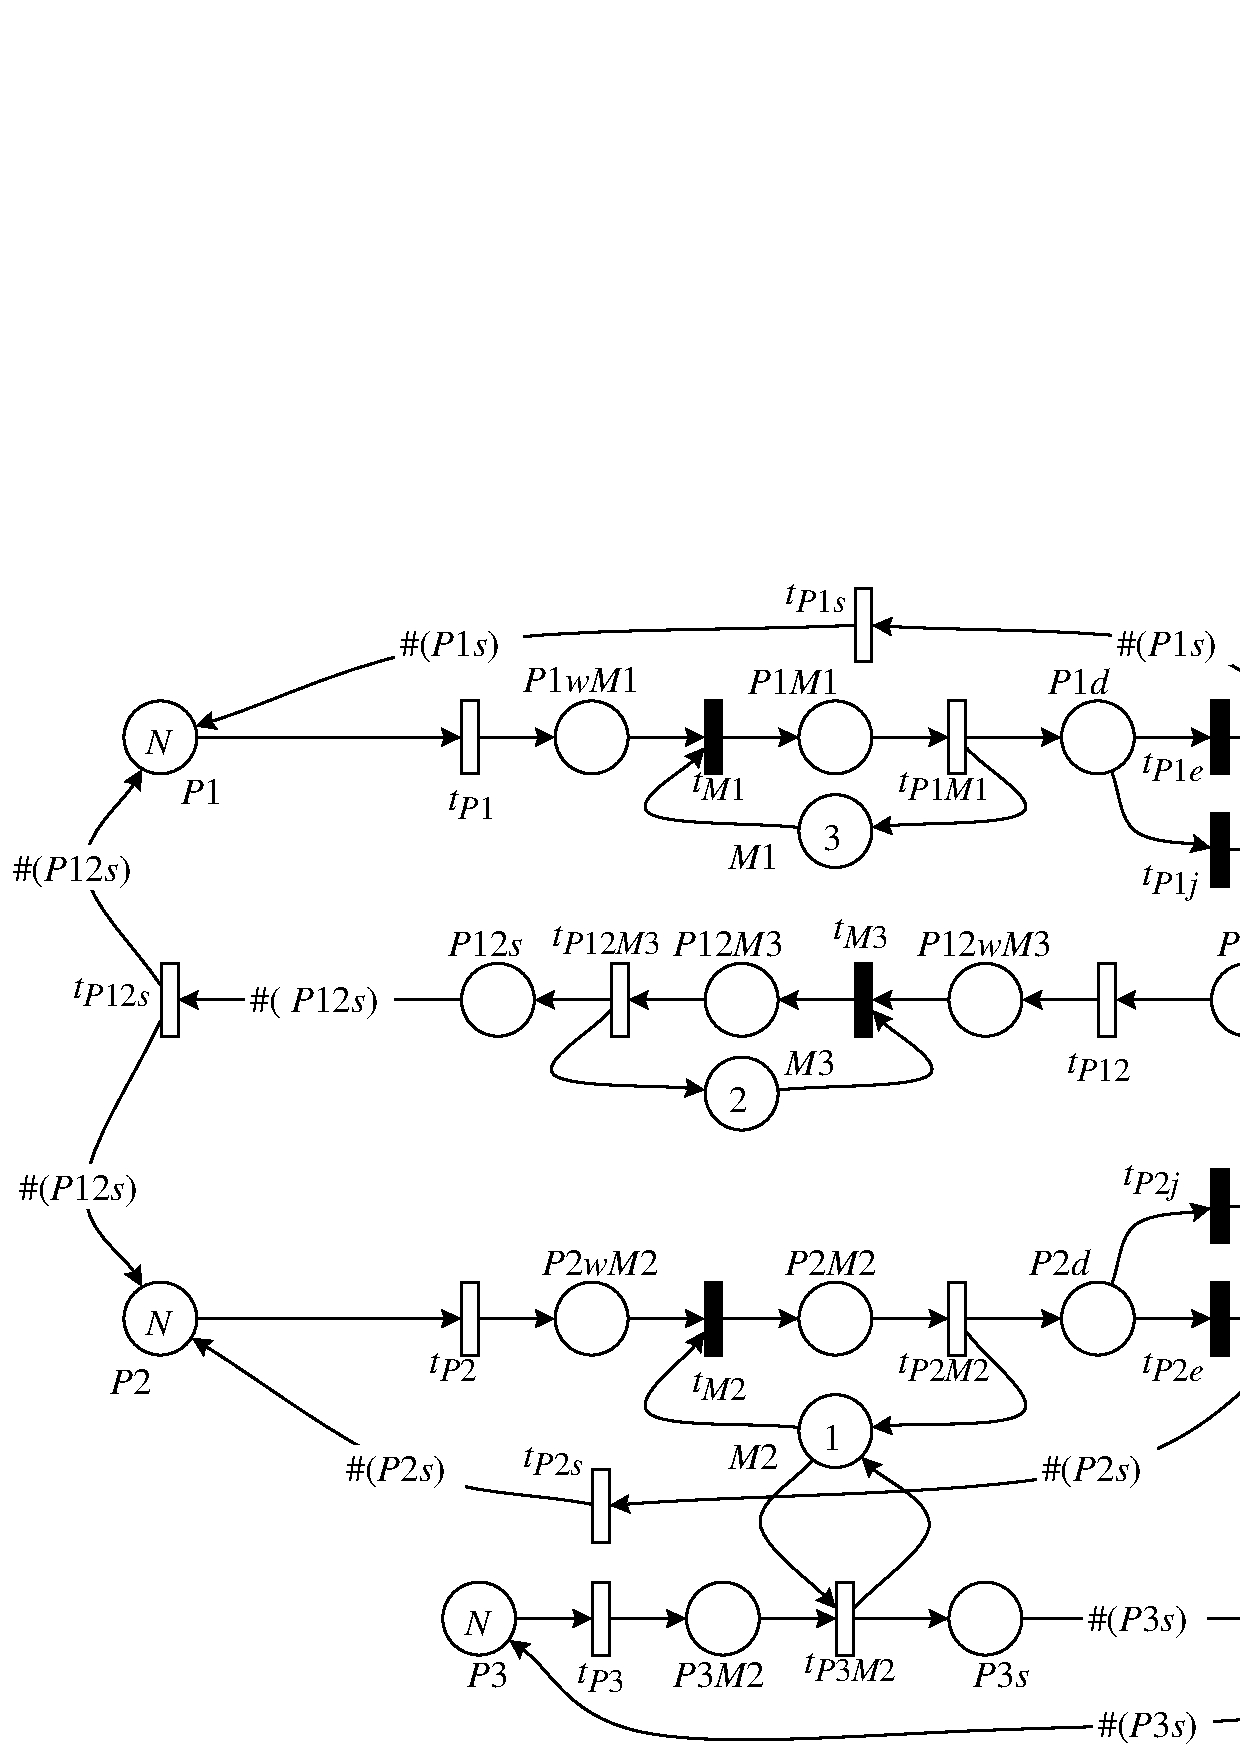
\includegraphics[scale=0.5]{figures/FMS-smartman.pdf}
  \caption{A flexible manufacturing system.}
  \label{FIG:fms}
\end{figure}


\begin{comment}

Had we wanted to use a structural solution approach, we could have
partitioned the model with the statement
\begin{code}
\begin{verbatim}
partition(P1:P1wM1:P1M1:M1:P1d:P1s, P12s:P12M3:M3:P12wM3:P12:P1wP2:P2wP1,
  P2:P2wM2:P2M2:M2:P2d:P2s, P3:P3M2:P3s);
\end{verbatim}
\end{code}
(which defines four submodels) and used the options
\begin{code}
\begin{verbatim}
# StateStorage MULTI_LEVEL_AVL
# MarkovStorage MATRIX_DIAGRAM_GENERAL
\end{verbatim}
\end{code}
Note, however, that the usually more efficient methods
\begin{code}
\begin{verbatim}
# StateStorage MDD_SATURATION
# MarkovStorage MATRIX_DIAGRAM_KRONECKER
\end{verbatim}
\end{code}
cannot be used with the given partition, because some immediate transitions,
such as \Code{tP1j}, are synchronizing (i.e., they affect multiple submodels).

%We partition the model into 19 levels obtained by assigning
%each place to a different level, with the exception of
%the complementary places $M_1$, $M_2$, and $M_3$, placed in the same level
%as the places $P_1M_1$, $P_2M_2$, and $P_{12}M_3$, respectively.

\end{comment}

%%%%%%%%%%%%%%%%%%%%%%%%%%%%%%%%%%%%%%%%%%%%%%%%%%%%%%%%%%%%%%%%%%%%%%%%%%%%
\section{Slotted ring}

Fig.~\ref{FIG:slotted} shows the Petri net for a single node of a slotted
ring network protocol \cite{Pastor1994}.
The overall model is composed of $N$
such subnets connected by merging transitions
(i.e., $\mathit{Free}_{(i+1) \bmod N}$ and $\mathit{Used}_{(i+1) \bmod N}$
really belong to the ``next'' subnet).
The following {\smart} code shows a decomposition where each
node of the ring is in a different level, and the requested
measure is simply the number of states.
%
\lstinputlisting[firstline=3]{examples/slot.sm}
%

\begin{figure}
  \centering
  \includegraphics[scale=0.5]{figures/slot.pdf}
  \caption{Model of a slotted ring.}
  \label{FIG:slotted}
\end{figure}


%%%%%%%%%%%%%%%%%%%%%%%%%%%%%%%%%%%%%%%%%%%%%%%%%%%%%%%%%%%%%%%%%%%%%%%%%%%%
\section{A Kanban system}

This model \cite{1996WMPN-SNSkanban}, shown in Fig.~\ref{FIG:kanban},
is parameterized by the number $N$ of tokens initially
in $p_{1}$, $p_{2}$, $p_{3}$, and $p_{4}$.
The following code shows a partition into four levels, one per kanban station.
The output measure is the number of arcs in the state-to-state transition
matrix for $N$ varying from $1$ to a maximum specified at runtime.
\begin{figure}
  \centering
  \includegraphics[scale=1]{figures/kanban.pdf}
  \caption{A kanban system.}
  \label{FIG:kanban}
\end{figure}
%
\lstinputlisting[firstline=3]{examples/kanban.sm}
%



%%%%%%%%%%%%%%%%%%%%%%%%%%%%%%%%%%%%%%%%%%%%%%%%%%%%%%%%%%%%%%%%%%%%%%%%%%%%
\section{Randomized leader election protocol}

The randomized asynchronous leader election protocol in \cite{DolevKR82}
solves the following problem: given a ring of $N$ processors, the
participants are required to designate a unique processor as leader by
sending messages around the ring. The ring is unidirectional, meaning that
the processes send messages to their unique successor (e.g. the one to the
right), and receive messages from their unique predecessor. It is known that
if the processors are indistinguishable (no unique identifiers are
assigned), then there is no deterministic algorithm to solve the problem.

The randomized algorithm works in phases. At the beginning of every round,
each process flips a coin to decide whether it will continue running for
election or not. Initially all processes are valid candidates. After
choosing a value ($0 = $ don't run this round, $1 = $ run), this is
communicated to the neighbour to the right. A process is eliminated from the
race only if it chose not to run and it's predecessor chose to run. After
being eliminated from the race, a process never becomes eligible again (it
enters the inactive state), and it is used only to relay messages between
active nodes around the ring. They do no initiate any communication.
Termination is detected by the active processes (at least one active node
exists at all times) by sending a token around the ring to count the
inactive nodes. The process that receives its own token with count $N-1$ is
the elected leader.

In our model, each processes has $5$ state variables:
\begin{lstlisting}
status[i]       : {start, wait, active, inactive, leader};      // init start
preference[i]   : {0, 1};                                       // init 0
counter[i]      : {0..N-1};                                     // init 0
sent[i]         : {none, pref, counter};                        // init none
recv[i]         : {none, pref, counter};                        // init none
\end{lstlisting}

\begin{figure}
  \centering
  \includegraphics[scale=0.5]{figures/leaderchart.pdf}
  \caption{State transition chart for the \Code{status} variable.}
  \label{FIG:leaderchart}
\end{figure}

\noindent The state-transition diagram for the \Code{status} of a process is
shown in Figure \ref{FIG:leaderchart}.

\IGNORE{
The Petri Net model is shown is Figure \ref{FIG:leaderfig}
\begin{figure}
  \CENTERPSSCALE{leaderfig}{0.5}
  \caption{Petri net model: the subnet of process $i$.}
  \label{FIG:leaderfig}
\end{figure}
}

\noindent The SMART code for this model is listed below:
%
\lstinputlisting[firstline=3]{examples/leader.sm}
%



%%%%%%%%%%%%%%%%%%%%%%%%%%%%%%%%%%%%%%%%%%%%%%%%%%%%%%%%%%%%%%%%%%%%%%%%%%%%
\section{A round--robin mutual exclusion protocol}

\begin{comment}
The protocol regulates the access to a shared resource (e.g. a communication
channel) for a ring of $N$ processors. The resource manager gives permission
to use the channel to each process in order, by moving a token around the
ring. When a process has the token, it reads in a message from the channel and
stores it in its own buffer. It can then release the token to the next processor 
before reading the contents of the buffer, or read the buffer first and then 
send the token to the neighbour.

Figure \ref{FIG:robinfig} shows the subnet for process $i$. 
Each subnet is initially marked with one token in place $\id{wait}_i$, 
except for process $0$ which starts with one token in $\id{req}_i$, meaning 
that it is the first process to have access when the protocol starts.

\begin{figure}
  \CENTERPSSCALE{robinfig}{0.5}
  \caption{The round--robin mutual exclusion.}
  \label{FIG:robinfig}
\end{figure}

\begin{code}
\begin{verbatim}
spn robin(int N) := {
  place Res;
  partition(1:Res);
  for (int i in {0..N-1}) {
    place
        R[i], bufidle[i], buffull[i],
        pwait[i], pask[i], pok[i], pload[i], psend[i];
    trans
        task[i], tbuf[i], t1load[i], t2load[i], t1send[i], t2send[i];
    partition(
        i+2:bufidle[i]:buffull[i]:pwait[i]:pask[i]:pok[i]:pload[i]:psend[i],
        1:R[i]);
    firing(task[i]:expo(1.0), tbuf[i]:expo(1.0), t1load[i]:expo(1.0),
        t1send[i]:expo(1.0), t2load[i]:expo(1.0), t2send[i]:expo(1.0));
  }
  for (int i in {0..N-1}) {
    arcs(Res:task[i], pask[i]:task[i], task[i]:R[i], task[i]:pok[i],
        R[i]:tbuf[i], bufidle[i]:tbuf[i], tbuf[i]:buffull[i], tbuf[i]:Res,
        buffull[i]:t1load[i], pok[i]:t1load[i], t1load[i]:bufidle[i], t1load[i]:psend[i],
        buffull[i]:t2load[i], pload[i]:t2load[i], t2load[i]:bufidle[i], t2load[i]:pwait[i],
        pok[i]:t1send[i], pwait[mod(i+1,N)]:t1send[i], 
        t1send[i]:pload[i], t1send[i]:pask[mod(i+1,N)],
        psend[i]:t2send[i], pwait[mod(i+1,N)]:t2send[i], 
        t2send[i]:pwait[i], t2send[i]:pask[mod(i+1,N)]);
  }
  init(Res:1, pask[0]:1);
  for (int i in {1..N-1}) {init (pwait[i]:1);}
  for (int i in {0..N-1}) {init(bufidle[i]:1);}
}
\end{verbatim}
\end{code}

\end{comment}


\appendix
% \input{appendix-language}
% \input{appendix-bnf}
% \input{appendix-phasetype}

\backmatter

\addcontentsline{toc}{chapter}{Bibliography}
\bibliographystyle{abbrv}
\bibliography{ALL}

% \addcontentsline{toc}{chapter}{Release notes}

% \newpage

% \input{releasenotes}

\PRIVATE{
\addcontentsline{toc}{chapter}{Index}
\printindex
}


\end{document}

